% Local IspellDict: english
% --------------------------------------------------------
% Reference Manual content
% copyright by BREDEX GmbH 2004
% --------------------------------------------------------

\title{Functional Testing Reference Manual}
%author is apparently necessary otherwise build fails. 
\author*{}{}
%\bxbanner{../../../share/PS/splash}
\maketitle
% ----------------------------------------------------------------------
%% % $Id: version.tex 7776 2009-01-30 17:08:26Z alexandra $
%% % Local Variables:
%% % ispell-check-comments: nil
%% % Local IspellDict: american
%% % End:
%% % --------------------------------------------------------
%% % User documentation
%% % copyright by BREDEX GmbH 2005
%% % --------------------------------------------------------
%% % this command can be inserted multiple times
%% \gdhelpid{}
%% % 
%% \begin{bxdescription}
%% \end{bxdescription}
%% %
%% \begin{bxsteps}
%% % use the \item command for single steps
%% \end{bxsteps}
%% % change <FILE> to the same filename you are editing
%% \bxinput{Links/<FILE>}
%% %
%% % other usefull commands are
%% %   \bxhint{}        to create a hint
%% %   \bxwarn{}        to describe a warning
\index{Project!Version}
\index{Versioning Projects}

\begin{enumerate}
\item To create a different version of a \gdproject{}, select:\\
\bxmenu{Test}{Create new version}{}.
\item An automatic suggestion for the next version number is provided.  
\item You can accept this version number or enter a different one.  
\item Click \bxcaption{OK} to create the new version. 
\item The new version of the \gdproject{} becomes active in the client. 
\bxtipp{Any test result summaries for the \gdproject{} are not duplicated in the new version. Tests that ran for previous versions of the \gdproject{} are, however, still in the \gddb{} to be used for long term analysis.}
\end{enumerate}
\bxtipp{You can also create a new version using the dbtool \bxpref{TasksDBToolCreateVersion}}

\bxdocinfo{RELEASE}{BREDEX GmbH}{\today}{}
%\bxdocinfo{RELEASE}{BREDEX GmbH}{\today}{}
\maxtocdepth{subsubsection}
\tableofcontents
% uncomment the following line to hide all \bxcomment's (i.e. for a
% release)
% FIXME MH: L2H doesn't like \renewcommand, find other solution
\renewcommand{\bxcomment}[2]{}%
% ----------------------------------------------------------------------
% set ToC depth for pdf, l2h handles this separately
\latexonly{\settocdepth{subsubsection}}
\clearpage

\chapter{Introduction}
The amount of keywords you have in a \app{} test and the amount of components your test deals with can grow very quickly. For this reason, it is important to think about structuring the \gdtestcasebrowser{} and the \gdomeditor{} to make finding \gdcases{} and component names easier. 


\subsection{Configuring task repositories in your workspace}
\label{TasksALMConfigureWorkspace}
Each repository you want to work with in your \ite{} must be configured in the workspace you are using. 

\begin{enumerate}
\item Select:\\ \bxmenu{Window}{Show View}{Other}\\ from the menu.
\item In the \bxname{Mylyn} section, select \bxname{Task Repositories} and click \bxcaption{OK}. The \bxname{Task Repositories} View will appear. The Bugzilla Repositories for \gd{} and \jb{} are pre-configured.
\item In the \bxname{Task Repositories} View, right click and select \bxname{Add Task Repository} from the context menu.
\item In the dialog that appears, you will see the pre-defined task repositories for the \ite{}. You can select one of these or choose to install a different connector. Depending on the connector you want to use, you may require additional software from Tasktop, or the connector may incur license fees.
\item Once you have selected your connector, click \bxcaption{Next}.
\item On the following page, you will need to configure the task repository. Please refer to the Mylyn documentation for information on repository configuration. 
\item Click \bxcaption{Finish} once the repository is configured.
\item To be able to see tasks in this repository, select: \\ \bxmenu{Window}{Show View}{Other}\\ from the menu. 
\item In the \bxname{Mylyn} section, select \bxname{Task List} and click \bxcaption{OK}. The \bxname{Task List} View will appear.
\end{enumerate}

You will now be able to see items in this repository, open them in the \ite{}, add queries for your workspace and work on tasks from this repository. 
You will also be able to select this repository in the \gdproject{} properties as the repository for your \gdproject{} \bxpref{TasksALMConfigureProject}. 


\subsection{Working on tasks in the \ite{}: contexts}
Once you have configured a task repository for your workspace \bxpref{TasksALMConfigureWorkspace}, you can work on tasks from that repository. 

\subsubsection{Opening and editing tasks in the \ite{}}
\begin{itemize}
\item To be able to see tasks in a repository, select: \\ \bxmenu{Window}{Show View}{Other}\\ from the menu. 
\item In the \bxname{Mylyn} section, select \bxname{Task List} and click \bxcaption{OK}. The \bxname{Task List} View will appear.
\item Double-click on a task to open this task in the editor area.
\item Once a task is open, you can work on it as you would in an external system -- add comments, change status etc.
\end{itemize}

\subsubsection{Working on tasks in the \ite{}}
\label{TasksActivateTask}
Mylyn supports context- or task-based working. When you work on a task, you only see items relevant to that task, so that coming back to the task later involves less context-switching. 
\begin{itemize}
\item Mylyn supports context-based working. You can work on existing tasks in a configured repository, or you can create tasks to work on.
\item To work on a task, you must \bxname{activate} it. To activate a task, select the task in the \bxname{Task List} and select:\\ \bxmenu{Activate}{}{}\\
from the context-sensitive menu. 
\item When you activate a task for the first time, the browsers and editors will seem very empty. This is because nothing is yet a part of the context for this task.
\item You can navigate through the browsers by pressing \bxkey{Alt+Click} to expand each level, or you can press the \bxname{Focus on task} button in the browsers to show the whole tree (not focusing on the task), or just the items in the current context (focusing on the task). 
\item Items are automatically added to your context when you select them in a browser, when you open them in an editor, or when you perform other actions that cause them to be made relevant (e.g. \gdcase{} creation, showing a \gdcase{} specification etc.). Items that are used particularly frequently are marked as \bxname{landmarks} and shown in bold. 
\item You can manually alter which items are in your context using the context-sensitive menu for a specific item. You can manually make items landmarks, or remove them from the context. 
\item The context that is created for you will be re-created when you reactivate the task at a later point. 
\end{itemize}



\subsection{Creating tasks in external repositories from test result reports}
\gdhelpid{testResultViewContextId}{Test Results View}
 You can create a new task with pre-filled information directly from an open test result report in the \gdtestresultview{}. This is useful if a test has failed and you want to create e.g. an issue in your bug-tracking system for the failure. 
\begin{enumerate}
\item In an open test result report, select the node that best describes the test failure (e.g. a \gdcase{} or \gdstep{} that has failed, or the whole \gdsuite{}, then right-click and select:\\
\bxmenu{Create a Mylyn Task}{}{}\\
from the context-sensitive menu.
\item  In the dialog that appears, select a repository in which to create the task. A \bxname{local} repository is available by default, but you can also add connections to Bugzilla and Trac repositories by clicking \bxcaption{Add Task Repository} in the New Task Dialog. Connectors to other repositories can also be added. See the Mylyn documentation for more details on adding repositories.
\item Click \bxcaption{Finish} once you have selected your repository. 
\item The editor for a new task will appear. It is pre-filled with information relevant to the node that you selected. Edit the task to make it descriptive enough for a bug report and save the editor. 
\item Once you have created a task, you can activate it to start saving your context for this task. See the later section \bxpref{TasksActivateTask} for details.
\end{enumerate}


\subsection{Configuring a task repository for your \gdproject{}}
\label{TasksALMConfigureProject}
Once you have configured one or more repositories for your workspace \bxpref{}, you can select one of these to be the test-relevant repository for your \gdproject{}. 

This will let you:
\begin{itemize}
\item Add a task ID from this repository to \gdcases{}, \gdsuites{}, and \gdjobs{} in the \gdproject{} to signify that this item is the test for this task \bxpref{TasksALMAddTask}.
\item Automatically report test results to the task defined when a test runs.
\item View the test results for the relevant item in the dashboard as a link from the task repository.
\end{itemize}

To configure a task repository for your \gdproject{}:

\begin{enumerate}
\item In the \gdproject{} Properties, select \bxname{Mylyn ALM} from the tree on the left \bxfigref{TasksALMProjectProperties}.
\item In the page that appears, you can select a repository from the combo-box.
\item You can then choose whether to only report failed tests, only report successful tests, or both.
\item Enter the URL of the \dash{} that is configured to use the correct \gddb{} for your test results. This is the \dash{} that will be opened when you click on a test result link from the task repository.
\end{enumerate}

\begin{figure}[h]
\begin{center}
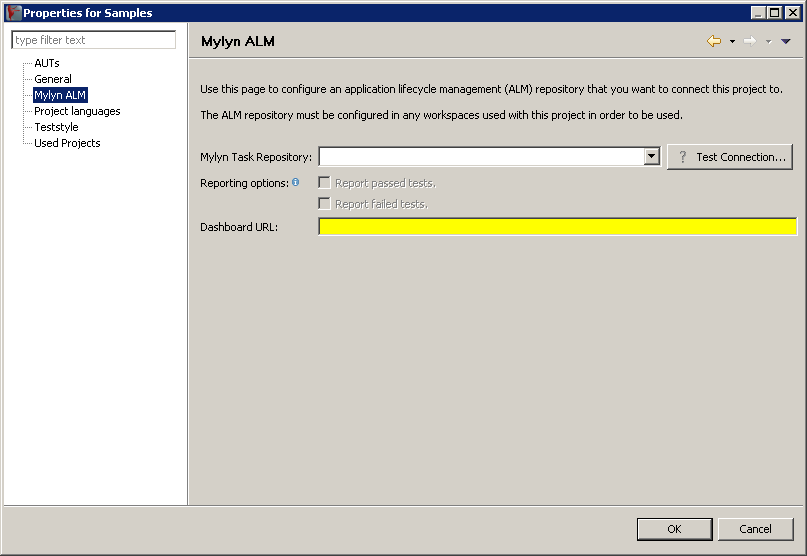
\includegraphics[width=12.5cm]{Tasks/ALM/PS/almproperties}
\caption{ALM Settings}
\label{TasksALMProjectProperties}
\end{center}
\end{figure}


\subsection{Adding task IDs to \gdjobs{}, \gdsuites{} and \gdcases{}}
\label{TasksALMAddTask}
You can add a task ID to \gdcases{}, \gdsuites{} and \gdjobs{} in your \gdproject{}. 

The task ID should be a valid ID in the repository that you have specified as the repository for this \gdproject{} \bxpref{TasksALMConfigureProject}. Adding the task ID to an item in your \gdproject{} means that this item is the relevant test for that task in your repository. When you activate the option, any test results for this item will be added as a comment to the task in the repository. The comment will include a link to the dashboard, in which the test result report can be viewed.

To add a task ID to a \gdcase{}, \gdsuite{} or \gdjob{}:
\begin{enumerate}
\item Open the item in the editor by double-clicking it.
\item In the \gdpropview{}, in the cell for \bxname{Task ID}, enter the task ID from the external repository. You can only enter task IDs at the place of specification -- you cannot overwrite them when you reuse the item.
\item Save the editor. 
\item When you have added a task ID to a node, you can open the task for this node from the browser by selecting:\\
\bxmenu{Open with}{Mylyn Task Editor}{}
\end{enumerate}

\bxtipp{You should ensure that you add task IDs to the right node-level to provide you with the relevant amount of information for the tasks in your repository. This will usually be at the level of Use Cases within a \gdsuite{}. }



\clearpage

\chapter{Shortcuts}
The amount of keywords you have in a \app{} test and the amount of components your test deals with can grow very quickly. For this reason, it is important to think about structuring the \gdtestcasebrowser{} and the \gdomeditor{} to make finding \gdcases{} and component names easier. 


\subsection{Configuring task repositories in your workspace}
\label{TasksALMConfigureWorkspace}
Each repository you want to work with in your \ite{} must be configured in the workspace you are using. 

\begin{enumerate}
\item Select:\\ \bxmenu{Window}{Show View}{Other}\\ from the menu.
\item In the \bxname{Mylyn} section, select \bxname{Task Repositories} and click \bxcaption{OK}. The \bxname{Task Repositories} View will appear. The Bugzilla Repositories for \gd{} and \jb{} are pre-configured.
\item In the \bxname{Task Repositories} View, right click and select \bxname{Add Task Repository} from the context menu.
\item In the dialog that appears, you will see the pre-defined task repositories for the \ite{}. You can select one of these or choose to install a different connector. Depending on the connector you want to use, you may require additional software from Tasktop, or the connector may incur license fees.
\item Once you have selected your connector, click \bxcaption{Next}.
\item On the following page, you will need to configure the task repository. Please refer to the Mylyn documentation for information on repository configuration. 
\item Click \bxcaption{Finish} once the repository is configured.
\item To be able to see tasks in this repository, select: \\ \bxmenu{Window}{Show View}{Other}\\ from the menu. 
\item In the \bxname{Mylyn} section, select \bxname{Task List} and click \bxcaption{OK}. The \bxname{Task List} View will appear.
\end{enumerate}

You will now be able to see items in this repository, open them in the \ite{}, add queries for your workspace and work on tasks from this repository. 
You will also be able to select this repository in the \gdproject{} properties as the repository for your \gdproject{} \bxpref{TasksALMConfigureProject}. 


\subsection{Working on tasks in the \ite{}: contexts}
Once you have configured a task repository for your workspace \bxpref{TasksALMConfigureWorkspace}, you can work on tasks from that repository. 

\subsubsection{Opening and editing tasks in the \ite{}}
\begin{itemize}
\item To be able to see tasks in a repository, select: \\ \bxmenu{Window}{Show View}{Other}\\ from the menu. 
\item In the \bxname{Mylyn} section, select \bxname{Task List} and click \bxcaption{OK}. The \bxname{Task List} View will appear.
\item Double-click on a task to open this task in the editor area.
\item Once a task is open, you can work on it as you would in an external system -- add comments, change status etc.
\end{itemize}

\subsubsection{Working on tasks in the \ite{}}
\label{TasksActivateTask}
Mylyn supports context- or task-based working. When you work on a task, you only see items relevant to that task, so that coming back to the task later involves less context-switching. 
\begin{itemize}
\item Mylyn supports context-based working. You can work on existing tasks in a configured repository, or you can create tasks to work on.
\item To work on a task, you must \bxname{activate} it. To activate a task, select the task in the \bxname{Task List} and select:\\ \bxmenu{Activate}{}{}\\
from the context-sensitive menu. 
\item When you activate a task for the first time, the browsers and editors will seem very empty. This is because nothing is yet a part of the context for this task.
\item You can navigate through the browsers by pressing \bxkey{Alt+Click} to expand each level, or you can press the \bxname{Focus on task} button in the browsers to show the whole tree (not focusing on the task), or just the items in the current context (focusing on the task). 
\item Items are automatically added to your context when you select them in a browser, when you open them in an editor, or when you perform other actions that cause them to be made relevant (e.g. \gdcase{} creation, showing a \gdcase{} specification etc.). Items that are used particularly frequently are marked as \bxname{landmarks} and shown in bold. 
\item You can manually alter which items are in your context using the context-sensitive menu for a specific item. You can manually make items landmarks, or remove them from the context. 
\item The context that is created for you will be re-created when you reactivate the task at a later point. 
\end{itemize}



\subsection{Creating tasks in external repositories from test result reports}
\gdhelpid{testResultViewContextId}{Test Results View}
 You can create a new task with pre-filled information directly from an open test result report in the \gdtestresultview{}. This is useful if a test has failed and you want to create e.g. an issue in your bug-tracking system for the failure. 
\begin{enumerate}
\item In an open test result report, select the node that best describes the test failure (e.g. a \gdcase{} or \gdstep{} that has failed, or the whole \gdsuite{}, then right-click and select:\\
\bxmenu{Create a Mylyn Task}{}{}\\
from the context-sensitive menu.
\item  In the dialog that appears, select a repository in which to create the task. A \bxname{local} repository is available by default, but you can also add connections to Bugzilla and Trac repositories by clicking \bxcaption{Add Task Repository} in the New Task Dialog. Connectors to other repositories can also be added. See the Mylyn documentation for more details on adding repositories.
\item Click \bxcaption{Finish} once you have selected your repository. 
\item The editor for a new task will appear. It is pre-filled with information relevant to the node that you selected. Edit the task to make it descriptive enough for a bug report and save the editor. 
\item Once you have created a task, you can activate it to start saving your context for this task. See the later section \bxpref{TasksActivateTask} for details.
\end{enumerate}


\subsection{Configuring a task repository for your \gdproject{}}
\label{TasksALMConfigureProject}
Once you have configured one or more repositories for your workspace \bxpref{}, you can select one of these to be the test-relevant repository for your \gdproject{}. 

This will let you:
\begin{itemize}
\item Add a task ID from this repository to \gdcases{}, \gdsuites{}, and \gdjobs{} in the \gdproject{} to signify that this item is the test for this task \bxpref{TasksALMAddTask}.
\item Automatically report test results to the task defined when a test runs.
\item View the test results for the relevant item in the dashboard as a link from the task repository.
\end{itemize}

To configure a task repository for your \gdproject{}:

\begin{enumerate}
\item In the \gdproject{} Properties, select \bxname{Mylyn ALM} from the tree on the left \bxfigref{TasksALMProjectProperties}.
\item In the page that appears, you can select a repository from the combo-box.
\item You can then choose whether to only report failed tests, only report successful tests, or both.
\item Enter the URL of the \dash{} that is configured to use the correct \gddb{} for your test results. This is the \dash{} that will be opened when you click on a test result link from the task repository.
\end{enumerate}

\begin{figure}[h]
\begin{center}
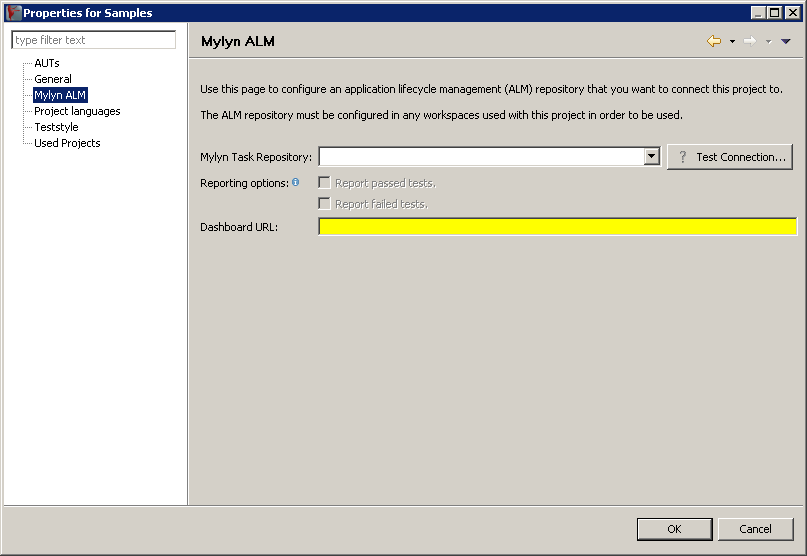
\includegraphics[width=12.5cm]{Tasks/ALM/PS/almproperties}
\caption{ALM Settings}
\label{TasksALMProjectProperties}
\end{center}
\end{figure}


\subsection{Adding task IDs to \gdjobs{}, \gdsuites{} and \gdcases{}}
\label{TasksALMAddTask}
You can add a task ID to \gdcases{}, \gdsuites{} and \gdjobs{} in your \gdproject{}. 

The task ID should be a valid ID in the repository that you have specified as the repository for this \gdproject{} \bxpref{TasksALMConfigureProject}. Adding the task ID to an item in your \gdproject{} means that this item is the relevant test for that task in your repository. When you activate the option, any test results for this item will be added as a comment to the task in the repository. The comment will include a link to the dashboard, in which the test result report can be viewed.

To add a task ID to a \gdcase{}, \gdsuite{} or \gdjob{}:
\begin{enumerate}
\item Open the item in the editor by double-clicking it.
\item In the \gdpropview{}, in the cell for \bxname{Task ID}, enter the task ID from the external repository. You can only enter task IDs at the place of specification -- you cannot overwrite them when you reuse the item.
\item Save the editor. 
\item When you have added a task ID to a node, you can open the task for this node from the browser by selecting:\\
\bxmenu{Open with}{Mylyn Task Editor}{}
\end{enumerate}

\bxtipp{You should ensure that you add task IDs to the right node-level to provide you with the relevant amount of information for the tasks in your repository. This will usually be at the level of Use Cases within a \gdsuite{}. }



\clearpage

\chapter{Using Regular Expressions for Text Verification}
\gdhelpid{guidancerPropertiesViewContextId}{Properties View}
\label{regex}
% $Id: Regex.tex 11851 2010-08-17 14:48:12Z alexandra $
% Local Variables:
% ispell-check-comments: nil
% Local IspellDict: american
% End:
% --------------------------------------------------------
% User documentation
% copyright by BREDEX GmbH 2005
% --------------------------------------------------------
\index{Regular Expressions}
% a helper macro to make things easier
% to describe a single element of regex syntax
\newcommand{\gdregex}[3]{%
#1 & #2 & #3 \\%
}%

\newcommand{\bxcarat}{\verb+^+}
\begin{itemize}
\item Using regular expressions lets you verify or select text even if you do not know exactly what the text is.
\item Using a system of placeholders for characters and some function symbols, you can enter a regular expression to find or check a text.
\item Actions which support regular expressions have an additional parameter, \bxcaption{Operator}. From this combo box, you can choose \bxcaption{matches}  to indicate that you want to use regular expressions.
\end{itemize}

\textbf{Simple matching}
\begin{itemize}
\item \bxshell{abc} matches \bxcaption{abc} and nothing else.
\end{itemize}

\textbf{Wildcards}
\begin{itemize}
\item \bxshell{.} represents one instance of any character.
\item \bxshell{..} represents two characters.  
\end{itemize}

\textbf{Repetition}
\begin{itemize}
\item Instead of using \bxshell{.} for each character, you can use symbols to indicate how many characters you are replacing with wildcards.
\item \bxshell{?} matches the previous character or group 0 or 1 time(s). E.g. \bxshell{a?} represents ''none or one \bxshell{a}''.
\item \bxshell{*} matches the previous character or group 0 or more time(s). E.g. \bxshell{a*} represents ''none or more \bxshell{a}''.
\item \bxshell{+} matches the previous character or group 1 or more time(s). E.g. \bxshell{a+} represents ''one or more \bxshell{a}''.
\item You can also use curly brackets \bxshell{\{\}}  to specify the minimum and maximum number of repetitions, e.g. \bxshell{\{4,7\}} looks for a minimum of four and a maximum of seven repetitions of the previous character.
\item To specify that a character must be repeated a minimum of four times, use: \bxshell{\{4,\}}
\end{itemize}

\textbf{Combining wildcards with repetition}
\begin{itemize}
\item You can specify a whole area of unknown text using \bxshell{.} and one of the repetition methods.
\item  \bxshell{.*} is an unlimited amount of any character, or none at all.
\item \bxshell{.?} is 0 or one of any character.
\item \bxshell{.+} is an unlimited amount of any character, but the character must appear at least once. 
\end{itemize}
\bxtipp{\jb{} applies your regular expression to your entire string. To search for a match within a string, wildcards need to be placed on either side. See the examples below for more information.}


\textbf{Ranges}
\begin{itemize}
\item For each individual character, you can specify a range of things it is allowed to be. 
\item A range is specified using square brackets (\bxshell{[]}) and a dash \bxshell{-}. 
\item For example, you can specify that a particular character can be any capital letter: \bxshell{[A-Z]}.
\end{itemize}
\bxtipp{Note that there are no spaces between the ranges. }

\textbf{Alternatives}
\begin{itemize}
\item Use a pipe ('{\tt |}') to specify alternatives.
\item For example, \bxshell{[a|b].*} will match a string that begins with \bxshell{a} or \bxshell{b}.
\end{itemize}

\textbf{Escape character}
\begin{itemize}
\item Backslash \bxshell{$\backslash$} is used to negate the effect of the character following the backslash.
\item The characters that are used to construct a regular expression need to be escaped if they are to be matched within a string.
\item The characters are: \newline
 \verb1 [ ] \ . | ? * + ( ) { } ^ $  1\newline 
\item Because \jb{} already uses a backslash as an escape symbol, you will need to use two backslashes to escape regular expression characters. 
\item For example, to check for a tree node:\\
\bxshell{x/y/z/***} \\
where the slashes are a part of the node, your regular expression in \jb{}  would look like this: \verb1 x\/y\/z\/\\*\\*\\* 1\newline
The backslashes before the ordinary slashes are an escape symbol to tell \jb{} that the following sign is not a path separator. The extra backslash before the stars tells \jb{} that the second backslash is to be interpreted as a backslash in the regular expression, i.e. as an escape symbol.  
\item E.g. If you want to check for a star (\bxshell{*}), then you have to enter \bxshell{$\backslash$$\backslash$*}. 
\end{itemize}

\textbf{Verbatim}
\begin{itemize}
\item You can avoid having to use multiple backslashes by putting the whole regular expression in single quotes:
\item The example above for a tree node could be entered thus:\\
\bxshell{'x/y/z/***'} 
\end{itemize}

\textbf{Useful examples}
\begin{itemize}
\item An empty field is represented by: \verb+^$+%$
\item A string that starts with \bxshell{a} is represented by: \bxshell{a.*}
\item A string that ends in \bxshell{a} is represented by: \bxshell{.*a}
\item A string that starts with \bxshell{a}, ends in \bxshell{b} and has unknown values (0 or more) in the middle is represented by: \bxshell{a.*b}
\item A string which contains \bxshell{a} somewhere between other unknown characters (0 or more) is represented by: \bxshell{.*a.*}
\item A password which can only contain capital letters and which must be between six and eight letters is represented by: \bxshell{[A-Z]\{6,8\}}.
\item A password which can contain any alphanumerical values and which must be at least six characters is represented by: \bxshell{[A-Za-z0-9]\{6,\}}.
\item You can check that a string corresponds to a minimum and maximum length using: \\
\verb#'^.{'={MIN_COUNT}','={MAX_COUNT}'}$'#
\item To check for a text which begins with a \bxshell{*}, you must use the escape character: \verb+\\*.*+
\end{itemize}

 
%% %In order to allow for powerful verification of textual data, \jb{}
%% %offers support for regular expressions conforming to the  
%% %\bxname{Perl 5} standard. In the actions which support regular
%% %expressions, there is an additional parameter which allows the user to
%% %activate/deactivate this feature.

%% %The following basic syntax can be applied for text verification with
%% %regular expressions:\bigskip

%% %% \begin{tabular}{p{1.5cm}p{5cm}p{2.5cm}}
%% %%   Syntax & Description & Example \\ \hline
%% %%   \jb{}efregex{letter, digit, etc.} {Except for a few special characters, \newline
%% %%     {\tt [ ] $\backslash$ . | ? * + ( ) } \newline
%% %%     entering any character will match itself. The above special
%% %%     characters are escaped with a backslash, {\tt $\backslash$ }. }
%% %%     {\bxshell{abc} matches \bxshell{abc}.
%% %%       }
%% %% \end{tabular}

%% \begin{description}
%%   \item[\textbf{simple matching}]
%%   To match a string exactly to that in a text field, simply type it in:

%%   \bxshell{abc} matches \bxshell{abc}, and nothing else.

%% %%   To specify that a string should appear at the beginning or end of a
%% %%   text, use a carat ('\verb.^.') or dollar sign ('{\tt \$}'), respectively:

%% %%   ''\verb.^.abc'' matches \bxshell{abcxxx} but not
%% %%   \bxshell{xabcxx}.
  
%% %%   \bxshell{abc\$} matches \bxshell{xxxabc} but not \bxshell{xxabcx}.
%%   \item[\textbf{character matching}]
%%   Use brackets ('{\tt [}' and '{\tt ]}') to specify a range of allowed
%%   characters at the current location. Ranges may also be given with a
%%   minus sign ('{\tt -}'),
%%   or alternatives with a ''pipe'' ('{\tt |}'). A period ('{\tt .}')
%%   may be used as a wildcard (instead of brackets) to match any
%%   single character.

%%   \bxshell{[0-9A-F]} matches the numbers zero through nine and the
%%   capital letters '{\tt A}' through '{\tt F}' but nothing else.

%%   \bxshell{a.b} matches \bxshell{azb} and \bxshell{a6b} but not
%%   \bxshell{ab}.

%%   Characters are grouped together using parentheses ('{\tt (}' and
%%   '{\tt )}').

%%   \item[\textbf{wildcards/repetition:}]
%%   Use '{\tt ?}' to match a character or group 0 or 1 time(s), '{\tt
%%   *}' to match 0 or more times, and '{\tt +}' to match 1 or more
%%   times. Numbers enclosed in brackets
%%  ('{\tt \{}' and '{\tt \}}') may be used  to specify the minimum and maximum
%%   repetitions. The expression

%%   ''\verb1abc.+xyz1''

%%   matches \bxshell{abcfghixyz} but not \bxshell{abcxyz}.

%%   Likewise, the expression

%%  ''\verb/[a-zA-Z][a-zA-Z0-9_\-]{4,7}/'' 

%%   may be used to
%%   verify a password format which accepts letters, numbers, '\verb/_/',
%%   and '{\tt -}', with a length between 5 and 8, where the first character
%%   must be a letter (note that '{\tt -}' is preceded by a backslash as
%%   an escape character, as it is normally used to specify range).

%% \end{description}

For additional information about syntax and usage of regular
expressions in general and in \jb{}{} in particular, please consult one
of the many textbooks on the subject.
%\bxcomment{MSH}{...or visit http://some.regex.site}
%\bxcomment{MSH}{Exactly what standard do these conform to?}

\clearpage

\chapter{Using Simple Match for Text Verification}
\gdhelpid{guidancerPropertiesViewContextId}{Properties View}
\label{simplematch}
% $Id: SimpleMatch.tex 7708 2009-01-20 15:50:45Z alexandra $
% Local Variables:
% ispell-check-comments: nil
% Local IspellDict: american
% End:
% --------------------------------------------------------
% User documentation
% copyright by BREDEX GmbH 2005
% --------------------------------------------------------
\index{Simple Match}


\begin{itemize}
\item Using \bxname{simple match} lets you verify or select text even if you do not know exactly what the text is.
\item Using a system of placeholders for characters and some function symbols, you can enter a simple match expression to find or check a text. The patterns for simple match are similar to Unix-style globs or Windows wildcards. The exact syntax is defined below.
\item Actions which support regular expressions have an additional parameter, \bxcaption{Operator}. From this combo box, you can choose \bxcaption{simple match} to indicate that you want to use simple matching.
\end{itemize}

\textbf{Simple matching}
\begin{itemize}
\item \bxshell{abc} matches \bxcaption{abc} and nothing else.
\end{itemize}

\textbf{Wildcards}
\begin{itemize}
\item \bxshell{?} represents one instance of any character.
\item \bxshell{*} represents any number (zero or more) of any characters.  
\end{itemize}

\bxtipp{\app{} applies your expression to your entire string. To search for a match within a string, wildcards need to be placed on either side. See the examples below for more information.}


\bxtipp{The following syntax information can be useful, but is also more complex. We recommend that simple match expressions use only letters (upper- and lowercase), numbers, and the wildcards described above. In this way, you can avoid complex syntax.}
\textbf{Ranges}
\begin{itemize}
\item For each individual character, you can specify a range of things it is allowed to be. 
\item A range is specified using square brackets (\bxshell{[]}) and a dash \bxshell{-}. 
\item For example, you can specify that a particular character can be any capital letter: \bxshell{[A-Z]}.
\end{itemize}

\textbf{Escape character}
\begin{itemize}
\item Backslash \bxshell{$\backslash$} is used to negate the effect of the character following the backslash.
\item The characters that are used to construct a simple match expression need to be escaped if they are to be matched within a string.
\item The characters are: \newline
 [ ? * \newline 
\item Because \app{} already uses a backslash as an escape symbol, you will need to use two backslashes to escape simple match characters. 
\item For example, to check for a tree node \bxcaption{x/y/z/***} where the slashes are a part of the node, your regular expression in \app{}  would look like this: \verb1 x\/y\/z\/\\*\\*\\* 1\newline
The backslashes before the ordinary slashes are an escape symbol to tell \app{} that the following sign is not a path separator. The extra backslash before the stars tells \app{} that the second backslash is to be interpreted as a backslash in the regular expression, i.e. as an escape symbol.  
\end{itemize}

\textbf{Useful examples}
\begin{itemize}
\item A string that starts with \bxshell{a} is represented by: \bxshell{a*}
\item A string that ends in \bxshell{a} is represented by: \bxshell{*a}
\item A string that starts with \bxshell{a}, ends in \bxshell{b} and has unknown values (0 or more) in the middle is represented by: \bxshell{a*b}
\item A string which contains \bxshell{a} somewhere between other unknown characters (0 or more) is represented by: \bxshell{*a*}
\item To check for a text which begins with a star (\bxshell{*}), you must use the escape character: \verb+\\**+
\end{itemize}
 

\clearpage

\latex{\settocdepth{subsubsection}} % subsubsection level
\chapter{Components, Actions, and Parameters}
 \label{actparam}
 The amount of keywords you have in a \app{} test and the amount of components your test deals with can grow very quickly. For this reason, it is important to think about structuring the \gdtestcasebrowser{} and the \gdomeditor{} to make finding \gdcases{} and component names easier. 


\subsection{Configuring task repositories in your workspace}
\label{TasksALMConfigureWorkspace}
Each repository you want to work with in your \ite{} must be configured in the workspace you are using. 

\begin{enumerate}
\item Select:\\ \bxmenu{Window}{Show View}{Other}\\ from the menu.
\item In the \bxname{Mylyn} section, select \bxname{Task Repositories} and click \bxcaption{OK}. The \bxname{Task Repositories} View will appear. The Bugzilla Repositories for \gd{} and \jb{} are pre-configured.
\item In the \bxname{Task Repositories} View, right click and select \bxname{Add Task Repository} from the context menu.
\item In the dialog that appears, you will see the pre-defined task repositories for the \ite{}. You can select one of these or choose to install a different connector. Depending on the connector you want to use, you may require additional software from Tasktop, or the connector may incur license fees.
\item Once you have selected your connector, click \bxcaption{Next}.
\item On the following page, you will need to configure the task repository. Please refer to the Mylyn documentation for information on repository configuration. 
\item Click \bxcaption{Finish} once the repository is configured.
\item To be able to see tasks in this repository, select: \\ \bxmenu{Window}{Show View}{Other}\\ from the menu. 
\item In the \bxname{Mylyn} section, select \bxname{Task List} and click \bxcaption{OK}. The \bxname{Task List} View will appear.
\end{enumerate}

You will now be able to see items in this repository, open them in the \ite{}, add queries for your workspace and work on tasks from this repository. 
You will also be able to select this repository in the \gdproject{} properties as the repository for your \gdproject{} \bxpref{TasksALMConfigureProject}. 


\subsection{Working on tasks in the \ite{}: contexts}
Once you have configured a task repository for your workspace \bxpref{TasksALMConfigureWorkspace}, you can work on tasks from that repository. 

\subsubsection{Opening and editing tasks in the \ite{}}
\begin{itemize}
\item To be able to see tasks in a repository, select: \\ \bxmenu{Window}{Show View}{Other}\\ from the menu. 
\item In the \bxname{Mylyn} section, select \bxname{Task List} and click \bxcaption{OK}. The \bxname{Task List} View will appear.
\item Double-click on a task to open this task in the editor area.
\item Once a task is open, you can work on it as you would in an external system -- add comments, change status etc.
\end{itemize}

\subsubsection{Working on tasks in the \ite{}}
\label{TasksActivateTask}
Mylyn supports context- or task-based working. When you work on a task, you only see items relevant to that task, so that coming back to the task later involves less context-switching. 
\begin{itemize}
\item Mylyn supports context-based working. You can work on existing tasks in a configured repository, or you can create tasks to work on.
\item To work on a task, you must \bxname{activate} it. To activate a task, select the task in the \bxname{Task List} and select:\\ \bxmenu{Activate}{}{}\\
from the context-sensitive menu. 
\item When you activate a task for the first time, the browsers and editors will seem very empty. This is because nothing is yet a part of the context for this task.
\item You can navigate through the browsers by pressing \bxkey{Alt+Click} to expand each level, or you can press the \bxname{Focus on task} button in the browsers to show the whole tree (not focusing on the task), or just the items in the current context (focusing on the task). 
\item Items are automatically added to your context when you select them in a browser, when you open them in an editor, or when you perform other actions that cause them to be made relevant (e.g. \gdcase{} creation, showing a \gdcase{} specification etc.). Items that are used particularly frequently are marked as \bxname{landmarks} and shown in bold. 
\item You can manually alter which items are in your context using the context-sensitive menu for a specific item. You can manually make items landmarks, or remove them from the context. 
\item The context that is created for you will be re-created when you reactivate the task at a later point. 
\end{itemize}



\subsection{Creating tasks in external repositories from test result reports}
\gdhelpid{testResultViewContextId}{Test Results View}
 You can create a new task with pre-filled information directly from an open test result report in the \gdtestresultview{}. This is useful if a test has failed and you want to create e.g. an issue in your bug-tracking system for the failure. 
\begin{enumerate}
\item In an open test result report, select the node that best describes the test failure (e.g. a \gdcase{} or \gdstep{} that has failed, or the whole \gdsuite{}, then right-click and select:\\
\bxmenu{Create a Mylyn Task}{}{}\\
from the context-sensitive menu.
\item  In the dialog that appears, select a repository in which to create the task. A \bxname{local} repository is available by default, but you can also add connections to Bugzilla and Trac repositories by clicking \bxcaption{Add Task Repository} in the New Task Dialog. Connectors to other repositories can also be added. See the Mylyn documentation for more details on adding repositories.
\item Click \bxcaption{Finish} once you have selected your repository. 
\item The editor for a new task will appear. It is pre-filled with information relevant to the node that you selected. Edit the task to make it descriptive enough for a bug report and save the editor. 
\item Once you have created a task, you can activate it to start saving your context for this task. See the later section \bxpref{TasksActivateTask} for details.
\end{enumerate}


\subsection{Configuring a task repository for your \gdproject{}}
\label{TasksALMConfigureProject}
Once you have configured one or more repositories for your workspace \bxpref{}, you can select one of these to be the test-relevant repository for your \gdproject{}. 

This will let you:
\begin{itemize}
\item Add a task ID from this repository to \gdcases{}, \gdsuites{}, and \gdjobs{} in the \gdproject{} to signify that this item is the test for this task \bxpref{TasksALMAddTask}.
\item Automatically report test results to the task defined when a test runs.
\item View the test results for the relevant item in the dashboard as a link from the task repository.
\end{itemize}

To configure a task repository for your \gdproject{}:

\begin{enumerate}
\item In the \gdproject{} Properties, select \bxname{Mylyn ALM} from the tree on the left \bxfigref{TasksALMProjectProperties}.
\item In the page that appears, you can select a repository from the combo-box.
\item You can then choose whether to only report failed tests, only report successful tests, or both.
\item Enter the URL of the \dash{} that is configured to use the correct \gddb{} for your test results. This is the \dash{} that will be opened when you click on a test result link from the task repository.
\end{enumerate}

\begin{figure}[h]
\begin{center}
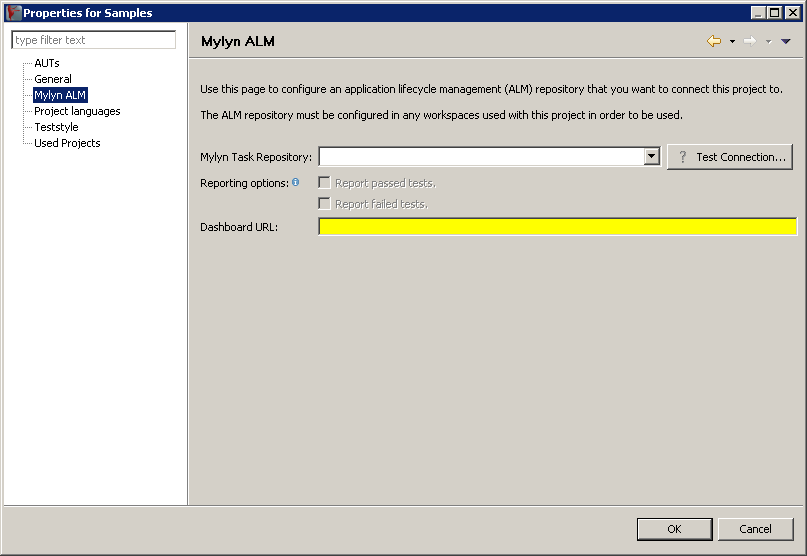
\includegraphics[width=12.5cm]{Tasks/ALM/PS/almproperties}
\caption{ALM Settings}
\label{TasksALMProjectProperties}
\end{center}
\end{figure}


\subsection{Adding task IDs to \gdjobs{}, \gdsuites{} and \gdcases{}}
\label{TasksALMAddTask}
You can add a task ID to \gdcases{}, \gdsuites{} and \gdjobs{} in your \gdproject{}. 

The task ID should be a valid ID in the repository that you have specified as the repository for this \gdproject{} \bxpref{TasksALMConfigureProject}. Adding the task ID to an item in your \gdproject{} means that this item is the relevant test for that task in your repository. When you activate the option, any test results for this item will be added as a comment to the task in the repository. The comment will include a link to the dashboard, in which the test result report can be viewed.

To add a task ID to a \gdcase{}, \gdsuite{} or \gdjob{}:
\begin{enumerate}
\item Open the item in the editor by double-clicking it.
\item In the \gdpropview{}, in the cell for \bxname{Task ID}, enter the task ID from the external repository. You can only enter task IDs at the place of specification -- you cannot overwrite them when you reuse the item.
\item Save the editor. 
\item When you have added a task ID to a node, you can open the task for this node from the browser by selecting:\\
\bxmenu{Open with}{Mylyn Task Editor}{}
\end{enumerate}

\bxtipp{You should ensure that you add task IDs to the right node-level to provide you with the relevant amount of information for the tasks in your repository. This will usually be at the level of Use Cases within a \gdsuite{}. }



 \clearpage

\latex{\settocdepth{subsubsection}}
\chapter{Constants for lists, combo boxes, trees and menus}
\label{constants}
The amount of keywords you have in a \app{} test and the amount of components your test deals with can grow very quickly. For this reason, it is important to think about structuring the \gdtestcasebrowser{} and the \gdomeditor{} to make finding \gdcases{} and component names easier. 


\subsection{Configuring task repositories in your workspace}
\label{TasksALMConfigureWorkspace}
Each repository you want to work with in your \ite{} must be configured in the workspace you are using. 

\begin{enumerate}
\item Select:\\ \bxmenu{Window}{Show View}{Other}\\ from the menu.
\item In the \bxname{Mylyn} section, select \bxname{Task Repositories} and click \bxcaption{OK}. The \bxname{Task Repositories} View will appear. The Bugzilla Repositories for \gd{} and \jb{} are pre-configured.
\item In the \bxname{Task Repositories} View, right click and select \bxname{Add Task Repository} from the context menu.
\item In the dialog that appears, you will see the pre-defined task repositories for the \ite{}. You can select one of these or choose to install a different connector. Depending on the connector you want to use, you may require additional software from Tasktop, or the connector may incur license fees.
\item Once you have selected your connector, click \bxcaption{Next}.
\item On the following page, you will need to configure the task repository. Please refer to the Mylyn documentation for information on repository configuration. 
\item Click \bxcaption{Finish} once the repository is configured.
\item To be able to see tasks in this repository, select: \\ \bxmenu{Window}{Show View}{Other}\\ from the menu. 
\item In the \bxname{Mylyn} section, select \bxname{Task List} and click \bxcaption{OK}. The \bxname{Task List} View will appear.
\end{enumerate}

You will now be able to see items in this repository, open them in the \ite{}, add queries for your workspace and work on tasks from this repository. 
You will also be able to select this repository in the \gdproject{} properties as the repository for your \gdproject{} \bxpref{TasksALMConfigureProject}. 


\subsection{Working on tasks in the \ite{}: contexts}
Once you have configured a task repository for your workspace \bxpref{TasksALMConfigureWorkspace}, you can work on tasks from that repository. 

\subsubsection{Opening and editing tasks in the \ite{}}
\begin{itemize}
\item To be able to see tasks in a repository, select: \\ \bxmenu{Window}{Show View}{Other}\\ from the menu. 
\item In the \bxname{Mylyn} section, select \bxname{Task List} and click \bxcaption{OK}. The \bxname{Task List} View will appear.
\item Double-click on a task to open this task in the editor area.
\item Once a task is open, you can work on it as you would in an external system -- add comments, change status etc.
\end{itemize}

\subsubsection{Working on tasks in the \ite{}}
\label{TasksActivateTask}
Mylyn supports context- or task-based working. When you work on a task, you only see items relevant to that task, so that coming back to the task later involves less context-switching. 
\begin{itemize}
\item Mylyn supports context-based working. You can work on existing tasks in a configured repository, or you can create tasks to work on.
\item To work on a task, you must \bxname{activate} it. To activate a task, select the task in the \bxname{Task List} and select:\\ \bxmenu{Activate}{}{}\\
from the context-sensitive menu. 
\item When you activate a task for the first time, the browsers and editors will seem very empty. This is because nothing is yet a part of the context for this task.
\item You can navigate through the browsers by pressing \bxkey{Alt+Click} to expand each level, or you can press the \bxname{Focus on task} button in the browsers to show the whole tree (not focusing on the task), or just the items in the current context (focusing on the task). 
\item Items are automatically added to your context when you select them in a browser, when you open them in an editor, or when you perform other actions that cause them to be made relevant (e.g. \gdcase{} creation, showing a \gdcase{} specification etc.). Items that are used particularly frequently are marked as \bxname{landmarks} and shown in bold. 
\item You can manually alter which items are in your context using the context-sensitive menu for a specific item. You can manually make items landmarks, or remove them from the context. 
\item The context that is created for you will be re-created when you reactivate the task at a later point. 
\end{itemize}



\subsection{Creating tasks in external repositories from test result reports}
\gdhelpid{testResultViewContextId}{Test Results View}
 You can create a new task with pre-filled information directly from an open test result report in the \gdtestresultview{}. This is useful if a test has failed and you want to create e.g. an issue in your bug-tracking system for the failure. 
\begin{enumerate}
\item In an open test result report, select the node that best describes the test failure (e.g. a \gdcase{} or \gdstep{} that has failed, or the whole \gdsuite{}, then right-click and select:\\
\bxmenu{Create a Mylyn Task}{}{}\\
from the context-sensitive menu.
\item  In the dialog that appears, select a repository in which to create the task. A \bxname{local} repository is available by default, but you can also add connections to Bugzilla and Trac repositories by clicking \bxcaption{Add Task Repository} in the New Task Dialog. Connectors to other repositories can also be added. See the Mylyn documentation for more details on adding repositories.
\item Click \bxcaption{Finish} once you have selected your repository. 
\item The editor for a new task will appear. It is pre-filled with information relevant to the node that you selected. Edit the task to make it descriptive enough for a bug report and save the editor. 
\item Once you have created a task, you can activate it to start saving your context for this task. See the later section \bxpref{TasksActivateTask} for details.
\end{enumerate}


\subsection{Configuring a task repository for your \gdproject{}}
\label{TasksALMConfigureProject}
Once you have configured one or more repositories for your workspace \bxpref{}, you can select one of these to be the test-relevant repository for your \gdproject{}. 

This will let you:
\begin{itemize}
\item Add a task ID from this repository to \gdcases{}, \gdsuites{}, and \gdjobs{} in the \gdproject{} to signify that this item is the test for this task \bxpref{TasksALMAddTask}.
\item Automatically report test results to the task defined when a test runs.
\item View the test results for the relevant item in the dashboard as a link from the task repository.
\end{itemize}

To configure a task repository for your \gdproject{}:

\begin{enumerate}
\item In the \gdproject{} Properties, select \bxname{Mylyn ALM} from the tree on the left \bxfigref{TasksALMProjectProperties}.
\item In the page that appears, you can select a repository from the combo-box.
\item You can then choose whether to only report failed tests, only report successful tests, or both.
\item Enter the URL of the \dash{} that is configured to use the correct \gddb{} for your test results. This is the \dash{} that will be opened when you click on a test result link from the task repository.
\end{enumerate}

\begin{figure}[h]
\begin{center}
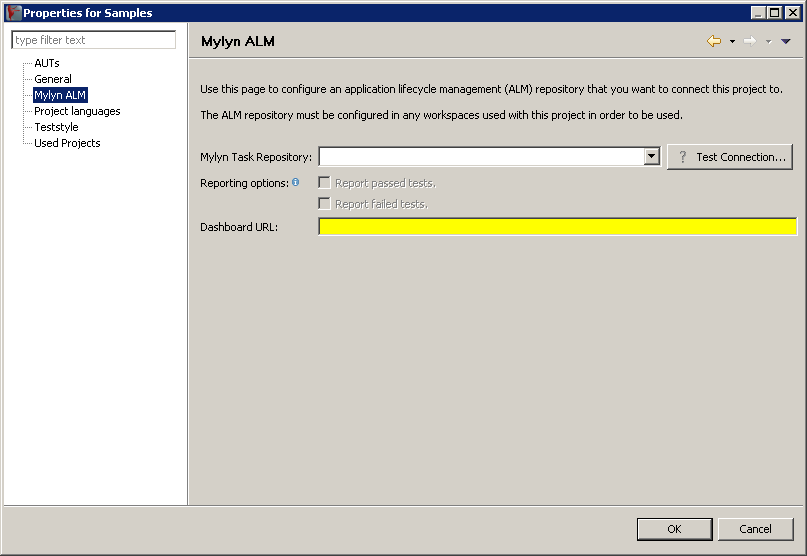
\includegraphics[width=12.5cm]{Tasks/ALM/PS/almproperties}
\caption{ALM Settings}
\label{TasksALMProjectProperties}
\end{center}
\end{figure}


\subsection{Adding task IDs to \gdjobs{}, \gdsuites{} and \gdcases{}}
\label{TasksALMAddTask}
You can add a task ID to \gdcases{}, \gdsuites{} and \gdjobs{} in your \gdproject{}. 

The task ID should be a valid ID in the repository that you have specified as the repository for this \gdproject{} \bxpref{TasksALMConfigureProject}. Adding the task ID to an item in your \gdproject{} means that this item is the relevant test for that task in your repository. When you activate the option, any test results for this item will be added as a comment to the task in the repository. The comment will include a link to the dashboard, in which the test result report can be viewed.

To add a task ID to a \gdcase{}, \gdsuite{} or \gdjob{}:
\begin{enumerate}
\item Open the item in the editor by double-clicking it.
\item In the \gdpropview{}, in the cell for \bxname{Task ID}, enter the task ID from the external repository. You can only enter task IDs at the place of specification -- you cannot overwrite them when you reuse the item.
\item Save the editor. 
\item When you have added a task ID to a node, you can open the task for this node from the browser by selecting:\\
\bxmenu{Open with}{Mylyn Task Editor}{}
\end{enumerate}

\bxtipp{You should ensure that you add task IDs to the right node-level to provide you with the relevant amount of information for the tasks in your repository. This will usually be at the level of Use Cases within a \gdsuite{}. }



\clearpage

\chapter{Overview of Components}
\label{overviewfam}
The amount of keywords you have in a \app{} test and the amount of components your test deals with can grow very quickly. For this reason, it is important to think about structuring the \gdtestcasebrowser{} and the \gdomeditor{} to make finding \gdcases{} and component names easier. 


\subsection{Configuring task repositories in your workspace}
\label{TasksALMConfigureWorkspace}
Each repository you want to work with in your \ite{} must be configured in the workspace you are using. 

\begin{enumerate}
\item Select:\\ \bxmenu{Window}{Show View}{Other}\\ from the menu.
\item In the \bxname{Mylyn} section, select \bxname{Task Repositories} and click \bxcaption{OK}. The \bxname{Task Repositories} View will appear. The Bugzilla Repositories for \gd{} and \jb{} are pre-configured.
\item In the \bxname{Task Repositories} View, right click and select \bxname{Add Task Repository} from the context menu.
\item In the dialog that appears, you will see the pre-defined task repositories for the \ite{}. You can select one of these or choose to install a different connector. Depending on the connector you want to use, you may require additional software from Tasktop, or the connector may incur license fees.
\item Once you have selected your connector, click \bxcaption{Next}.
\item On the following page, you will need to configure the task repository. Please refer to the Mylyn documentation for information on repository configuration. 
\item Click \bxcaption{Finish} once the repository is configured.
\item To be able to see tasks in this repository, select: \\ \bxmenu{Window}{Show View}{Other}\\ from the menu. 
\item In the \bxname{Mylyn} section, select \bxname{Task List} and click \bxcaption{OK}. The \bxname{Task List} View will appear.
\end{enumerate}

You will now be able to see items in this repository, open them in the \ite{}, add queries for your workspace and work on tasks from this repository. 
You will also be able to select this repository in the \gdproject{} properties as the repository for your \gdproject{} \bxpref{TasksALMConfigureProject}. 


\subsection{Working on tasks in the \ite{}: contexts}
Once you have configured a task repository for your workspace \bxpref{TasksALMConfigureWorkspace}, you can work on tasks from that repository. 

\subsubsection{Opening and editing tasks in the \ite{}}
\begin{itemize}
\item To be able to see tasks in a repository, select: \\ \bxmenu{Window}{Show View}{Other}\\ from the menu. 
\item In the \bxname{Mylyn} section, select \bxname{Task List} and click \bxcaption{OK}. The \bxname{Task List} View will appear.
\item Double-click on a task to open this task in the editor area.
\item Once a task is open, you can work on it as you would in an external system -- add comments, change status etc.
\end{itemize}

\subsubsection{Working on tasks in the \ite{}}
\label{TasksActivateTask}
Mylyn supports context- or task-based working. When you work on a task, you only see items relevant to that task, so that coming back to the task later involves less context-switching. 
\begin{itemize}
\item Mylyn supports context-based working. You can work on existing tasks in a configured repository, or you can create tasks to work on.
\item To work on a task, you must \bxname{activate} it. To activate a task, select the task in the \bxname{Task List} and select:\\ \bxmenu{Activate}{}{}\\
from the context-sensitive menu. 
\item When you activate a task for the first time, the browsers and editors will seem very empty. This is because nothing is yet a part of the context for this task.
\item You can navigate through the browsers by pressing \bxkey{Alt+Click} to expand each level, or you can press the \bxname{Focus on task} button in the browsers to show the whole tree (not focusing on the task), or just the items in the current context (focusing on the task). 
\item Items are automatically added to your context when you select them in a browser, when you open them in an editor, or when you perform other actions that cause them to be made relevant (e.g. \gdcase{} creation, showing a \gdcase{} specification etc.). Items that are used particularly frequently are marked as \bxname{landmarks} and shown in bold. 
\item You can manually alter which items are in your context using the context-sensitive menu for a specific item. You can manually make items landmarks, or remove them from the context. 
\item The context that is created for you will be re-created when you reactivate the task at a later point. 
\end{itemize}



\subsection{Creating tasks in external repositories from test result reports}
\gdhelpid{testResultViewContextId}{Test Results View}
 You can create a new task with pre-filled information directly from an open test result report in the \gdtestresultview{}. This is useful if a test has failed and you want to create e.g. an issue in your bug-tracking system for the failure. 
\begin{enumerate}
\item In an open test result report, select the node that best describes the test failure (e.g. a \gdcase{} or \gdstep{} that has failed, or the whole \gdsuite{}, then right-click and select:\\
\bxmenu{Create a Mylyn Task}{}{}\\
from the context-sensitive menu.
\item  In the dialog that appears, select a repository in which to create the task. A \bxname{local} repository is available by default, but you can also add connections to Bugzilla and Trac repositories by clicking \bxcaption{Add Task Repository} in the New Task Dialog. Connectors to other repositories can also be added. See the Mylyn documentation for more details on adding repositories.
\item Click \bxcaption{Finish} once you have selected your repository. 
\item The editor for a new task will appear. It is pre-filled with information relevant to the node that you selected. Edit the task to make it descriptive enough for a bug report and save the editor. 
\item Once you have created a task, you can activate it to start saving your context for this task. See the later section \bxpref{TasksActivateTask} for details.
\end{enumerate}


\subsection{Configuring a task repository for your \gdproject{}}
\label{TasksALMConfigureProject}
Once you have configured one or more repositories for your workspace \bxpref{}, you can select one of these to be the test-relevant repository for your \gdproject{}. 

This will let you:
\begin{itemize}
\item Add a task ID from this repository to \gdcases{}, \gdsuites{}, and \gdjobs{} in the \gdproject{} to signify that this item is the test for this task \bxpref{TasksALMAddTask}.
\item Automatically report test results to the task defined when a test runs.
\item View the test results for the relevant item in the dashboard as a link from the task repository.
\end{itemize}

To configure a task repository for your \gdproject{}:

\begin{enumerate}
\item In the \gdproject{} Properties, select \bxname{Mylyn ALM} from the tree on the left \bxfigref{TasksALMProjectProperties}.
\item In the page that appears, you can select a repository from the combo-box.
\item You can then choose whether to only report failed tests, only report successful tests, or both.
\item Enter the URL of the \dash{} that is configured to use the correct \gddb{} for your test results. This is the \dash{} that will be opened when you click on a test result link from the task repository.
\end{enumerate}

\begin{figure}[h]
\begin{center}
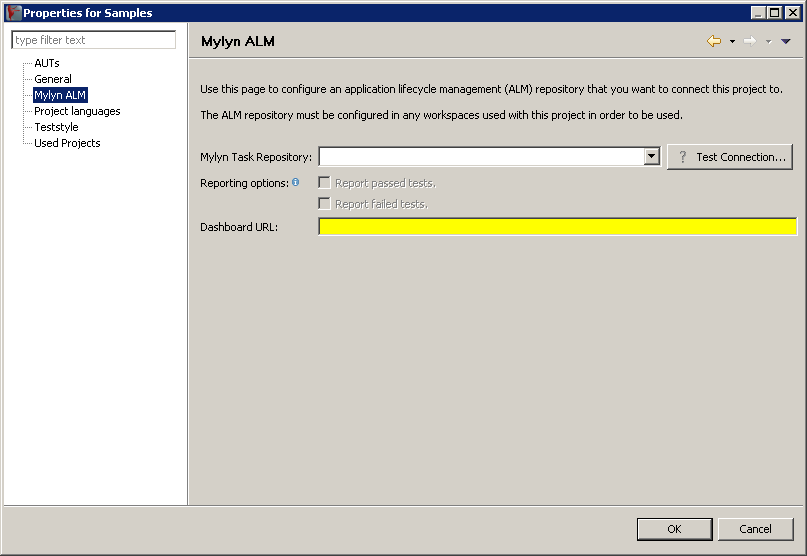
\includegraphics[width=12.5cm]{Tasks/ALM/PS/almproperties}
\caption{ALM Settings}
\label{TasksALMProjectProperties}
\end{center}
\end{figure}


\subsection{Adding task IDs to \gdjobs{}, \gdsuites{} and \gdcases{}}
\label{TasksALMAddTask}
You can add a task ID to \gdcases{}, \gdsuites{} and \gdjobs{} in your \gdproject{}. 

The task ID should be a valid ID in the repository that you have specified as the repository for this \gdproject{} \bxpref{TasksALMConfigureProject}. Adding the task ID to an item in your \gdproject{} means that this item is the relevant test for that task in your repository. When you activate the option, any test results for this item will be added as a comment to the task in the repository. The comment will include a link to the dashboard, in which the test result report can be viewed.

To add a task ID to a \gdcase{}, \gdsuite{} or \gdjob{}:
\begin{enumerate}
\item Open the item in the editor by double-clicking it.
\item In the \gdpropview{}, in the cell for \bxname{Task ID}, enter the task ID from the external repository. You can only enter task IDs at the place of specification -- you cannot overwrite them when you reuse the item.
\item Save the editor. 
\item When you have added a task ID to a node, you can open the task for this node from the browser by selecting:\\
\bxmenu{Open with}{Mylyn Task Editor}{}
\end{enumerate}

\bxtipp{You should ensure that you add task IDs to the right node-level to provide you with the relevant amount of information for the tasks in your repository. This will usually be at the level of Use Cases within a \gdsuite{}. }



\clearpage

\chapter{Using Relative Paths}
\gdhelpid{guidancerPropertiesViewContextId}{Properties View}
\gdhelpid{autConfigSettingWizardPagePageContextId}{Configuring an AUT}
\gdhelpid{autConfigPropDialogContextId}{AUT Configuration Settings}
\label{relativepath}
The amount of keywords you have in a \app{} test and the amount of components your test deals with can grow very quickly. For this reason, it is important to think about structuring the \gdtestcasebrowser{} and the \gdomeditor{} to make finding \gdcases{} and component names easier. 


\subsection{Configuring task repositories in your workspace}
\label{TasksALMConfigureWorkspace}
Each repository you want to work with in your \ite{} must be configured in the workspace you are using. 

\begin{enumerate}
\item Select:\\ \bxmenu{Window}{Show View}{Other}\\ from the menu.
\item In the \bxname{Mylyn} section, select \bxname{Task Repositories} and click \bxcaption{OK}. The \bxname{Task Repositories} View will appear. The Bugzilla Repositories for \gd{} and \jb{} are pre-configured.
\item In the \bxname{Task Repositories} View, right click and select \bxname{Add Task Repository} from the context menu.
\item In the dialog that appears, you will see the pre-defined task repositories for the \ite{}. You can select one of these or choose to install a different connector. Depending on the connector you want to use, you may require additional software from Tasktop, or the connector may incur license fees.
\item Once you have selected your connector, click \bxcaption{Next}.
\item On the following page, you will need to configure the task repository. Please refer to the Mylyn documentation for information on repository configuration. 
\item Click \bxcaption{Finish} once the repository is configured.
\item To be able to see tasks in this repository, select: \\ \bxmenu{Window}{Show View}{Other}\\ from the menu. 
\item In the \bxname{Mylyn} section, select \bxname{Task List} and click \bxcaption{OK}. The \bxname{Task List} View will appear.
\end{enumerate}

You will now be able to see items in this repository, open them in the \ite{}, add queries for your workspace and work on tasks from this repository. 
You will also be able to select this repository in the \gdproject{} properties as the repository for your \gdproject{} \bxpref{TasksALMConfigureProject}. 


\subsection{Working on tasks in the \ite{}: contexts}
Once you have configured a task repository for your workspace \bxpref{TasksALMConfigureWorkspace}, you can work on tasks from that repository. 

\subsubsection{Opening and editing tasks in the \ite{}}
\begin{itemize}
\item To be able to see tasks in a repository, select: \\ \bxmenu{Window}{Show View}{Other}\\ from the menu. 
\item In the \bxname{Mylyn} section, select \bxname{Task List} and click \bxcaption{OK}. The \bxname{Task List} View will appear.
\item Double-click on a task to open this task in the editor area.
\item Once a task is open, you can work on it as you would in an external system -- add comments, change status etc.
\end{itemize}

\subsubsection{Working on tasks in the \ite{}}
\label{TasksActivateTask}
Mylyn supports context- or task-based working. When you work on a task, you only see items relevant to that task, so that coming back to the task later involves less context-switching. 
\begin{itemize}
\item Mylyn supports context-based working. You can work on existing tasks in a configured repository, or you can create tasks to work on.
\item To work on a task, you must \bxname{activate} it. To activate a task, select the task in the \bxname{Task List} and select:\\ \bxmenu{Activate}{}{}\\
from the context-sensitive menu. 
\item When you activate a task for the first time, the browsers and editors will seem very empty. This is because nothing is yet a part of the context for this task.
\item You can navigate through the browsers by pressing \bxkey{Alt+Click} to expand each level, or you can press the \bxname{Focus on task} button in the browsers to show the whole tree (not focusing on the task), or just the items in the current context (focusing on the task). 
\item Items are automatically added to your context when you select them in a browser, when you open them in an editor, or when you perform other actions that cause them to be made relevant (e.g. \gdcase{} creation, showing a \gdcase{} specification etc.). Items that are used particularly frequently are marked as \bxname{landmarks} and shown in bold. 
\item You can manually alter which items are in your context using the context-sensitive menu for a specific item. You can manually make items landmarks, or remove them from the context. 
\item The context that is created for you will be re-created when you reactivate the task at a later point. 
\end{itemize}



\subsection{Creating tasks in external repositories from test result reports}
\gdhelpid{testResultViewContextId}{Test Results View}
 You can create a new task with pre-filled information directly from an open test result report in the \gdtestresultview{}. This is useful if a test has failed and you want to create e.g. an issue in your bug-tracking system for the failure. 
\begin{enumerate}
\item In an open test result report, select the node that best describes the test failure (e.g. a \gdcase{} or \gdstep{} that has failed, or the whole \gdsuite{}, then right-click and select:\\
\bxmenu{Create a Mylyn Task}{}{}\\
from the context-sensitive menu.
\item  In the dialog that appears, select a repository in which to create the task. A \bxname{local} repository is available by default, but you can also add connections to Bugzilla and Trac repositories by clicking \bxcaption{Add Task Repository} in the New Task Dialog. Connectors to other repositories can also be added. See the Mylyn documentation for more details on adding repositories.
\item Click \bxcaption{Finish} once you have selected your repository. 
\item The editor for a new task will appear. It is pre-filled with information relevant to the node that you selected. Edit the task to make it descriptive enough for a bug report and save the editor. 
\item Once you have created a task, you can activate it to start saving your context for this task. See the later section \bxpref{TasksActivateTask} for details.
\end{enumerate}


\subsection{Configuring a task repository for your \gdproject{}}
\label{TasksALMConfigureProject}
Once you have configured one or more repositories for your workspace \bxpref{}, you can select one of these to be the test-relevant repository for your \gdproject{}. 

This will let you:
\begin{itemize}
\item Add a task ID from this repository to \gdcases{}, \gdsuites{}, and \gdjobs{} in the \gdproject{} to signify that this item is the test for this task \bxpref{TasksALMAddTask}.
\item Automatically report test results to the task defined when a test runs.
\item View the test results for the relevant item in the dashboard as a link from the task repository.
\end{itemize}

To configure a task repository for your \gdproject{}:

\begin{enumerate}
\item In the \gdproject{} Properties, select \bxname{Mylyn ALM} from the tree on the left \bxfigref{TasksALMProjectProperties}.
\item In the page that appears, you can select a repository from the combo-box.
\item You can then choose whether to only report failed tests, only report successful tests, or both.
\item Enter the URL of the \dash{} that is configured to use the correct \gddb{} for your test results. This is the \dash{} that will be opened when you click on a test result link from the task repository.
\end{enumerate}

\begin{figure}[h]
\begin{center}
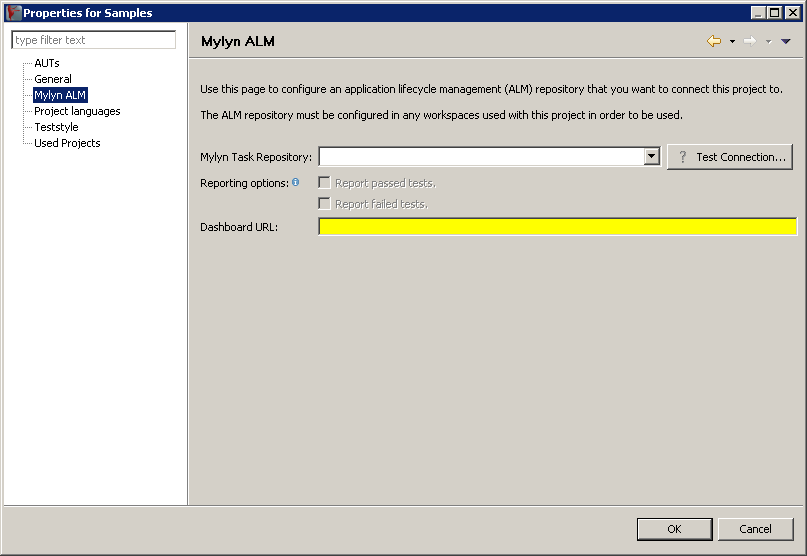
\includegraphics[width=12.5cm]{Tasks/ALM/PS/almproperties}
\caption{ALM Settings}
\label{TasksALMProjectProperties}
\end{center}
\end{figure}


\subsection{Adding task IDs to \gdjobs{}, \gdsuites{} and \gdcases{}}
\label{TasksALMAddTask}
You can add a task ID to \gdcases{}, \gdsuites{} and \gdjobs{} in your \gdproject{}. 

The task ID should be a valid ID in the repository that you have specified as the repository for this \gdproject{} \bxpref{TasksALMConfigureProject}. Adding the task ID to an item in your \gdproject{} means that this item is the relevant test for that task in your repository. When you activate the option, any test results for this item will be added as a comment to the task in the repository. The comment will include a link to the dashboard, in which the test result report can be viewed.

To add a task ID to a \gdcase{}, \gdsuite{} or \gdjob{}:
\begin{enumerate}
\item Open the item in the editor by double-clicking it.
\item In the \gdpropview{}, in the cell for \bxname{Task ID}, enter the task ID from the external repository. You can only enter task IDs at the place of specification -- you cannot overwrite them when you reuse the item.
\item Save the editor. 
\item When you have added a task ID to a node, you can open the task for this node from the browser by selecting:\\
\bxmenu{Open with}{Mylyn Task Editor}{}
\end{enumerate}

\bxtipp{You should ensure that you add task IDs to the right node-level to provide you with the relevant amount of information for the tasks in your repository. This will usually be at the level of Use Cases within a \gdsuite{}. }



\clearpage

\chapter{Special characters}
\gdhelpid{guidancerPropertiesViewContextId}{Properties View}
\gdhelpid{guidancerDataSetViewContextId}{Data Sets View}
\label{specialchar}
The amount of keywords you have in a \app{} test and the amount of components your test deals with can grow very quickly. For this reason, it is important to think about structuring the \gdtestcasebrowser{} and the \gdomeditor{} to make finding \gdcases{} and component names easier. 


\subsection{Configuring task repositories in your workspace}
\label{TasksALMConfigureWorkspace}
Each repository you want to work with in your \ite{} must be configured in the workspace you are using. 

\begin{enumerate}
\item Select:\\ \bxmenu{Window}{Show View}{Other}\\ from the menu.
\item In the \bxname{Mylyn} section, select \bxname{Task Repositories} and click \bxcaption{OK}. The \bxname{Task Repositories} View will appear. The Bugzilla Repositories for \gd{} and \jb{} are pre-configured.
\item In the \bxname{Task Repositories} View, right click and select \bxname{Add Task Repository} from the context menu.
\item In the dialog that appears, you will see the pre-defined task repositories for the \ite{}. You can select one of these or choose to install a different connector. Depending on the connector you want to use, you may require additional software from Tasktop, or the connector may incur license fees.
\item Once you have selected your connector, click \bxcaption{Next}.
\item On the following page, you will need to configure the task repository. Please refer to the Mylyn documentation for information on repository configuration. 
\item Click \bxcaption{Finish} once the repository is configured.
\item To be able to see tasks in this repository, select: \\ \bxmenu{Window}{Show View}{Other}\\ from the menu. 
\item In the \bxname{Mylyn} section, select \bxname{Task List} and click \bxcaption{OK}. The \bxname{Task List} View will appear.
\end{enumerate}

You will now be able to see items in this repository, open them in the \ite{}, add queries for your workspace and work on tasks from this repository. 
You will also be able to select this repository in the \gdproject{} properties as the repository for your \gdproject{} \bxpref{TasksALMConfigureProject}. 


\subsection{Working on tasks in the \ite{}: contexts}
Once you have configured a task repository for your workspace \bxpref{TasksALMConfigureWorkspace}, you can work on tasks from that repository. 

\subsubsection{Opening and editing tasks in the \ite{}}
\begin{itemize}
\item To be able to see tasks in a repository, select: \\ \bxmenu{Window}{Show View}{Other}\\ from the menu. 
\item In the \bxname{Mylyn} section, select \bxname{Task List} and click \bxcaption{OK}. The \bxname{Task List} View will appear.
\item Double-click on a task to open this task in the editor area.
\item Once a task is open, you can work on it as you would in an external system -- add comments, change status etc.
\end{itemize}

\subsubsection{Working on tasks in the \ite{}}
\label{TasksActivateTask}
Mylyn supports context- or task-based working. When you work on a task, you only see items relevant to that task, so that coming back to the task later involves less context-switching. 
\begin{itemize}
\item Mylyn supports context-based working. You can work on existing tasks in a configured repository, or you can create tasks to work on.
\item To work on a task, you must \bxname{activate} it. To activate a task, select the task in the \bxname{Task List} and select:\\ \bxmenu{Activate}{}{}\\
from the context-sensitive menu. 
\item When you activate a task for the first time, the browsers and editors will seem very empty. This is because nothing is yet a part of the context for this task.
\item You can navigate through the browsers by pressing \bxkey{Alt+Click} to expand each level, or you can press the \bxname{Focus on task} button in the browsers to show the whole tree (not focusing on the task), or just the items in the current context (focusing on the task). 
\item Items are automatically added to your context when you select them in a browser, when you open them in an editor, or when you perform other actions that cause them to be made relevant (e.g. \gdcase{} creation, showing a \gdcase{} specification etc.). Items that are used particularly frequently are marked as \bxname{landmarks} and shown in bold. 
\item You can manually alter which items are in your context using the context-sensitive menu for a specific item. You can manually make items landmarks, or remove them from the context. 
\item The context that is created for you will be re-created when you reactivate the task at a later point. 
\end{itemize}



\subsection{Creating tasks in external repositories from test result reports}
\gdhelpid{testResultViewContextId}{Test Results View}
 You can create a new task with pre-filled information directly from an open test result report in the \gdtestresultview{}. This is useful if a test has failed and you want to create e.g. an issue in your bug-tracking system for the failure. 
\begin{enumerate}
\item In an open test result report, select the node that best describes the test failure (e.g. a \gdcase{} or \gdstep{} that has failed, or the whole \gdsuite{}, then right-click and select:\\
\bxmenu{Create a Mylyn Task}{}{}\\
from the context-sensitive menu.
\item  In the dialog that appears, select a repository in which to create the task. A \bxname{local} repository is available by default, but you can also add connections to Bugzilla and Trac repositories by clicking \bxcaption{Add Task Repository} in the New Task Dialog. Connectors to other repositories can also be added. See the Mylyn documentation for more details on adding repositories.
\item Click \bxcaption{Finish} once you have selected your repository. 
\item The editor for a new task will appear. It is pre-filled with information relevant to the node that you selected. Edit the task to make it descriptive enough for a bug report and save the editor. 
\item Once you have created a task, you can activate it to start saving your context for this task. See the later section \bxpref{TasksActivateTask} for details.
\end{enumerate}


\subsection{Configuring a task repository for your \gdproject{}}
\label{TasksALMConfigureProject}
Once you have configured one or more repositories for your workspace \bxpref{}, you can select one of these to be the test-relevant repository for your \gdproject{}. 

This will let you:
\begin{itemize}
\item Add a task ID from this repository to \gdcases{}, \gdsuites{}, and \gdjobs{} in the \gdproject{} to signify that this item is the test for this task \bxpref{TasksALMAddTask}.
\item Automatically report test results to the task defined when a test runs.
\item View the test results for the relevant item in the dashboard as a link from the task repository.
\end{itemize}

To configure a task repository for your \gdproject{}:

\begin{enumerate}
\item In the \gdproject{} Properties, select \bxname{Mylyn ALM} from the tree on the left \bxfigref{TasksALMProjectProperties}.
\item In the page that appears, you can select a repository from the combo-box.
\item You can then choose whether to only report failed tests, only report successful tests, or both.
\item Enter the URL of the \dash{} that is configured to use the correct \gddb{} for your test results. This is the \dash{} that will be opened when you click on a test result link from the task repository.
\end{enumerate}

\begin{figure}[h]
\begin{center}
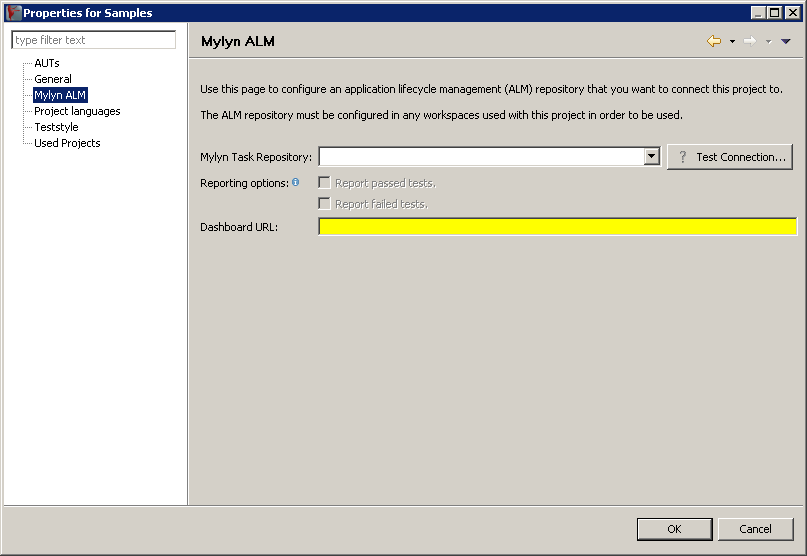
\includegraphics[width=12.5cm]{Tasks/ALM/PS/almproperties}
\caption{ALM Settings}
\label{TasksALMProjectProperties}
\end{center}
\end{figure}


\subsection{Adding task IDs to \gdjobs{}, \gdsuites{} and \gdcases{}}
\label{TasksALMAddTask}
You can add a task ID to \gdcases{}, \gdsuites{} and \gdjobs{} in your \gdproject{}. 

The task ID should be a valid ID in the repository that you have specified as the repository for this \gdproject{} \bxpref{TasksALMConfigureProject}. Adding the task ID to an item in your \gdproject{} means that this item is the relevant test for that task in your repository. When you activate the option, any test results for this item will be added as a comment to the task in the repository. The comment will include a link to the dashboard, in which the test result report can be viewed.

To add a task ID to a \gdcase{}, \gdsuite{} or \gdjob{}:
\begin{enumerate}
\item Open the item in the editor by double-clicking it.
\item In the \gdpropview{}, in the cell for \bxname{Task ID}, enter the task ID from the external repository. You can only enter task IDs at the place of specification -- you cannot overwrite them when you reuse the item.
\item Save the editor. 
\item When you have added a task ID to a node, you can open the task for this node from the browser by selecting:\\
\bxmenu{Open with}{Mylyn Task Editor}{}
\end{enumerate}

\bxtipp{You should ensure that you add task IDs to the right node-level to provide you with the relevant amount of information for the tasks in your repository. This will usually be at the level of Use Cases within a \gdsuite{}. }



\clearpage

\chapter{Language Codes}
\label{langcodes}
The amount of keywords you have in a \app{} test and the amount of components your test deals with can grow very quickly. For this reason, it is important to think about structuring the \gdtestcasebrowser{} and the \gdomeditor{} to make finding \gdcases{} and component names easier. 


\subsection{Configuring task repositories in your workspace}
\label{TasksALMConfigureWorkspace}
Each repository you want to work with in your \ite{} must be configured in the workspace you are using. 

\begin{enumerate}
\item Select:\\ \bxmenu{Window}{Show View}{Other}\\ from the menu.
\item In the \bxname{Mylyn} section, select \bxname{Task Repositories} and click \bxcaption{OK}. The \bxname{Task Repositories} View will appear. The Bugzilla Repositories for \gd{} and \jb{} are pre-configured.
\item In the \bxname{Task Repositories} View, right click and select \bxname{Add Task Repository} from the context menu.
\item In the dialog that appears, you will see the pre-defined task repositories for the \ite{}. You can select one of these or choose to install a different connector. Depending on the connector you want to use, you may require additional software from Tasktop, or the connector may incur license fees.
\item Once you have selected your connector, click \bxcaption{Next}.
\item On the following page, you will need to configure the task repository. Please refer to the Mylyn documentation for information on repository configuration. 
\item Click \bxcaption{Finish} once the repository is configured.
\item To be able to see tasks in this repository, select: \\ \bxmenu{Window}{Show View}{Other}\\ from the menu. 
\item In the \bxname{Mylyn} section, select \bxname{Task List} and click \bxcaption{OK}. The \bxname{Task List} View will appear.
\end{enumerate}

You will now be able to see items in this repository, open them in the \ite{}, add queries for your workspace and work on tasks from this repository. 
You will also be able to select this repository in the \gdproject{} properties as the repository for your \gdproject{} \bxpref{TasksALMConfigureProject}. 


\subsection{Working on tasks in the \ite{}: contexts}
Once you have configured a task repository for your workspace \bxpref{TasksALMConfigureWorkspace}, you can work on tasks from that repository. 

\subsubsection{Opening and editing tasks in the \ite{}}
\begin{itemize}
\item To be able to see tasks in a repository, select: \\ \bxmenu{Window}{Show View}{Other}\\ from the menu. 
\item In the \bxname{Mylyn} section, select \bxname{Task List} and click \bxcaption{OK}. The \bxname{Task List} View will appear.
\item Double-click on a task to open this task in the editor area.
\item Once a task is open, you can work on it as you would in an external system -- add comments, change status etc.
\end{itemize}

\subsubsection{Working on tasks in the \ite{}}
\label{TasksActivateTask}
Mylyn supports context- or task-based working. When you work on a task, you only see items relevant to that task, so that coming back to the task later involves less context-switching. 
\begin{itemize}
\item Mylyn supports context-based working. You can work on existing tasks in a configured repository, or you can create tasks to work on.
\item To work on a task, you must \bxname{activate} it. To activate a task, select the task in the \bxname{Task List} and select:\\ \bxmenu{Activate}{}{}\\
from the context-sensitive menu. 
\item When you activate a task for the first time, the browsers and editors will seem very empty. This is because nothing is yet a part of the context for this task.
\item You can navigate through the browsers by pressing \bxkey{Alt+Click} to expand each level, or you can press the \bxname{Focus on task} button in the browsers to show the whole tree (not focusing on the task), or just the items in the current context (focusing on the task). 
\item Items are automatically added to your context when you select them in a browser, when you open them in an editor, or when you perform other actions that cause them to be made relevant (e.g. \gdcase{} creation, showing a \gdcase{} specification etc.). Items that are used particularly frequently are marked as \bxname{landmarks} and shown in bold. 
\item You can manually alter which items are in your context using the context-sensitive menu for a specific item. You can manually make items landmarks, or remove them from the context. 
\item The context that is created for you will be re-created when you reactivate the task at a later point. 
\end{itemize}



\subsection{Creating tasks in external repositories from test result reports}
\gdhelpid{testResultViewContextId}{Test Results View}
 You can create a new task with pre-filled information directly from an open test result report in the \gdtestresultview{}. This is useful if a test has failed and you want to create e.g. an issue in your bug-tracking system for the failure. 
\begin{enumerate}
\item In an open test result report, select the node that best describes the test failure (e.g. a \gdcase{} or \gdstep{} that has failed, or the whole \gdsuite{}, then right-click and select:\\
\bxmenu{Create a Mylyn Task}{}{}\\
from the context-sensitive menu.
\item  In the dialog that appears, select a repository in which to create the task. A \bxname{local} repository is available by default, but you can also add connections to Bugzilla and Trac repositories by clicking \bxcaption{Add Task Repository} in the New Task Dialog. Connectors to other repositories can also be added. See the Mylyn documentation for more details on adding repositories.
\item Click \bxcaption{Finish} once you have selected your repository. 
\item The editor for a new task will appear. It is pre-filled with information relevant to the node that you selected. Edit the task to make it descriptive enough for a bug report and save the editor. 
\item Once you have created a task, you can activate it to start saving your context for this task. See the later section \bxpref{TasksActivateTask} for details.
\end{enumerate}


\subsection{Configuring a task repository for your \gdproject{}}
\label{TasksALMConfigureProject}
Once you have configured one or more repositories for your workspace \bxpref{}, you can select one of these to be the test-relevant repository for your \gdproject{}. 

This will let you:
\begin{itemize}
\item Add a task ID from this repository to \gdcases{}, \gdsuites{}, and \gdjobs{} in the \gdproject{} to signify that this item is the test for this task \bxpref{TasksALMAddTask}.
\item Automatically report test results to the task defined when a test runs.
\item View the test results for the relevant item in the dashboard as a link from the task repository.
\end{itemize}

To configure a task repository for your \gdproject{}:

\begin{enumerate}
\item In the \gdproject{} Properties, select \bxname{Mylyn ALM} from the tree on the left \bxfigref{TasksALMProjectProperties}.
\item In the page that appears, you can select a repository from the combo-box.
\item You can then choose whether to only report failed tests, only report successful tests, or both.
\item Enter the URL of the \dash{} that is configured to use the correct \gddb{} for your test results. This is the \dash{} that will be opened when you click on a test result link from the task repository.
\end{enumerate}

\begin{figure}[h]
\begin{center}
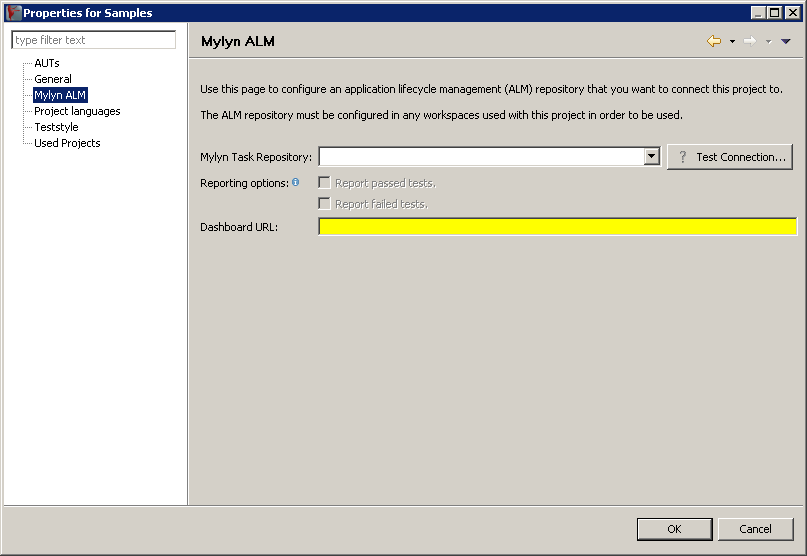
\includegraphics[width=12.5cm]{Tasks/ALM/PS/almproperties}
\caption{ALM Settings}
\label{TasksALMProjectProperties}
\end{center}
\end{figure}


\subsection{Adding task IDs to \gdjobs{}, \gdsuites{} and \gdcases{}}
\label{TasksALMAddTask}
You can add a task ID to \gdcases{}, \gdsuites{} and \gdjobs{} in your \gdproject{}. 

The task ID should be a valid ID in the repository that you have specified as the repository for this \gdproject{} \bxpref{TasksALMConfigureProject}. Adding the task ID to an item in your \gdproject{} means that this item is the relevant test for that task in your repository. When you activate the option, any test results for this item will be added as a comment to the task in the repository. The comment will include a link to the dashboard, in which the test result report can be viewed.

To add a task ID to a \gdcase{}, \gdsuite{} or \gdjob{}:
\begin{enumerate}
\item Open the item in the editor by double-clicking it.
\item In the \gdpropview{}, in the cell for \bxname{Task ID}, enter the task ID from the external repository. You can only enter task IDs at the place of specification -- you cannot overwrite them when you reuse the item.
\item Save the editor. 
\item When you have added a task ID to a node, you can open the task for this node from the browser by selecting:\\
\bxmenu{Open with}{Mylyn Task Editor}{}
\end{enumerate}

\bxtipp{You should ensure that you add task IDs to the right node-level to provide you with the relevant amount of information for the tasks in your repository. This will usually be at the level of Use Cases within a \gdsuite{}. }



\clearpage

\chapter{Keyboard layout files}
\label{keyboardlayout}
The amount of keywords you have in a \app{} test and the amount of components your test deals with can grow very quickly. For this reason, it is important to think about structuring the \gdtestcasebrowser{} and the \gdomeditor{} to make finding \gdcases{} and component names easier. 


\subsection{Configuring task repositories in your workspace}
\label{TasksALMConfigureWorkspace}
Each repository you want to work with in your \ite{} must be configured in the workspace you are using. 

\begin{enumerate}
\item Select:\\ \bxmenu{Window}{Show View}{Other}\\ from the menu.
\item In the \bxname{Mylyn} section, select \bxname{Task Repositories} and click \bxcaption{OK}. The \bxname{Task Repositories} View will appear. The Bugzilla Repositories for \gd{} and \jb{} are pre-configured.
\item In the \bxname{Task Repositories} View, right click and select \bxname{Add Task Repository} from the context menu.
\item In the dialog that appears, you will see the pre-defined task repositories for the \ite{}. You can select one of these or choose to install a different connector. Depending on the connector you want to use, you may require additional software from Tasktop, or the connector may incur license fees.
\item Once you have selected your connector, click \bxcaption{Next}.
\item On the following page, you will need to configure the task repository. Please refer to the Mylyn documentation for information on repository configuration. 
\item Click \bxcaption{Finish} once the repository is configured.
\item To be able to see tasks in this repository, select: \\ \bxmenu{Window}{Show View}{Other}\\ from the menu. 
\item In the \bxname{Mylyn} section, select \bxname{Task List} and click \bxcaption{OK}. The \bxname{Task List} View will appear.
\end{enumerate}

You will now be able to see items in this repository, open them in the \ite{}, add queries for your workspace and work on tasks from this repository. 
You will also be able to select this repository in the \gdproject{} properties as the repository for your \gdproject{} \bxpref{TasksALMConfigureProject}. 


\subsection{Working on tasks in the \ite{}: contexts}
Once you have configured a task repository for your workspace \bxpref{TasksALMConfigureWorkspace}, you can work on tasks from that repository. 

\subsubsection{Opening and editing tasks in the \ite{}}
\begin{itemize}
\item To be able to see tasks in a repository, select: \\ \bxmenu{Window}{Show View}{Other}\\ from the menu. 
\item In the \bxname{Mylyn} section, select \bxname{Task List} and click \bxcaption{OK}. The \bxname{Task List} View will appear.
\item Double-click on a task to open this task in the editor area.
\item Once a task is open, you can work on it as you would in an external system -- add comments, change status etc.
\end{itemize}

\subsubsection{Working on tasks in the \ite{}}
\label{TasksActivateTask}
Mylyn supports context- or task-based working. When you work on a task, you only see items relevant to that task, so that coming back to the task later involves less context-switching. 
\begin{itemize}
\item Mylyn supports context-based working. You can work on existing tasks in a configured repository, or you can create tasks to work on.
\item To work on a task, you must \bxname{activate} it. To activate a task, select the task in the \bxname{Task List} and select:\\ \bxmenu{Activate}{}{}\\
from the context-sensitive menu. 
\item When you activate a task for the first time, the browsers and editors will seem very empty. This is because nothing is yet a part of the context for this task.
\item You can navigate through the browsers by pressing \bxkey{Alt+Click} to expand each level, or you can press the \bxname{Focus on task} button in the browsers to show the whole tree (not focusing on the task), or just the items in the current context (focusing on the task). 
\item Items are automatically added to your context when you select them in a browser, when you open them in an editor, or when you perform other actions that cause them to be made relevant (e.g. \gdcase{} creation, showing a \gdcase{} specification etc.). Items that are used particularly frequently are marked as \bxname{landmarks} and shown in bold. 
\item You can manually alter which items are in your context using the context-sensitive menu for a specific item. You can manually make items landmarks, or remove them from the context. 
\item The context that is created for you will be re-created when you reactivate the task at a later point. 
\end{itemize}



\subsection{Creating tasks in external repositories from test result reports}
\gdhelpid{testResultViewContextId}{Test Results View}
 You can create a new task with pre-filled information directly from an open test result report in the \gdtestresultview{}. This is useful if a test has failed and you want to create e.g. an issue in your bug-tracking system for the failure. 
\begin{enumerate}
\item In an open test result report, select the node that best describes the test failure (e.g. a \gdcase{} or \gdstep{} that has failed, or the whole \gdsuite{}, then right-click and select:\\
\bxmenu{Create a Mylyn Task}{}{}\\
from the context-sensitive menu.
\item  In the dialog that appears, select a repository in which to create the task. A \bxname{local} repository is available by default, but you can also add connections to Bugzilla and Trac repositories by clicking \bxcaption{Add Task Repository} in the New Task Dialog. Connectors to other repositories can also be added. See the Mylyn documentation for more details on adding repositories.
\item Click \bxcaption{Finish} once you have selected your repository. 
\item The editor for a new task will appear. It is pre-filled with information relevant to the node that you selected. Edit the task to make it descriptive enough for a bug report and save the editor. 
\item Once you have created a task, you can activate it to start saving your context for this task. See the later section \bxpref{TasksActivateTask} for details.
\end{enumerate}


\subsection{Configuring a task repository for your \gdproject{}}
\label{TasksALMConfigureProject}
Once you have configured one or more repositories for your workspace \bxpref{}, you can select one of these to be the test-relevant repository for your \gdproject{}. 

This will let you:
\begin{itemize}
\item Add a task ID from this repository to \gdcases{}, \gdsuites{}, and \gdjobs{} in the \gdproject{} to signify that this item is the test for this task \bxpref{TasksALMAddTask}.
\item Automatically report test results to the task defined when a test runs.
\item View the test results for the relevant item in the dashboard as a link from the task repository.
\end{itemize}

To configure a task repository for your \gdproject{}:

\begin{enumerate}
\item In the \gdproject{} Properties, select \bxname{Mylyn ALM} from the tree on the left \bxfigref{TasksALMProjectProperties}.
\item In the page that appears, you can select a repository from the combo-box.
\item You can then choose whether to only report failed tests, only report successful tests, or both.
\item Enter the URL of the \dash{} that is configured to use the correct \gddb{} for your test results. This is the \dash{} that will be opened when you click on a test result link from the task repository.
\end{enumerate}

\begin{figure}[h]
\begin{center}
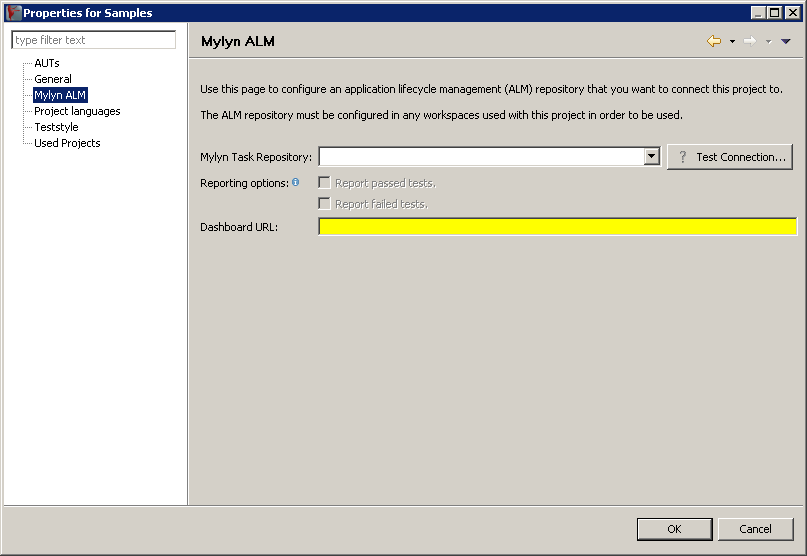
\includegraphics[width=12.5cm]{Tasks/ALM/PS/almproperties}
\caption{ALM Settings}
\label{TasksALMProjectProperties}
\end{center}
\end{figure}


\subsection{Adding task IDs to \gdjobs{}, \gdsuites{} and \gdcases{}}
\label{TasksALMAddTask}
You can add a task ID to \gdcases{}, \gdsuites{} and \gdjobs{} in your \gdproject{}. 

The task ID should be a valid ID in the repository that you have specified as the repository for this \gdproject{} \bxpref{TasksALMConfigureProject}. Adding the task ID to an item in your \gdproject{} means that this item is the relevant test for that task in your repository. When you activate the option, any test results for this item will be added as a comment to the task in the repository. The comment will include a link to the dashboard, in which the test result report can be viewed.

To add a task ID to a \gdcase{}, \gdsuite{} or \gdjob{}:
\begin{enumerate}
\item Open the item in the editor by double-clicking it.
\item In the \gdpropview{}, in the cell for \bxname{Task ID}, enter the task ID from the external repository. You can only enter task IDs at the place of specification -- you cannot overwrite them when you reuse the item.
\item Save the editor. 
\item When you have added a task ID to a node, you can open the task for this node from the browser by selecting:\\
\bxmenu{Open with}{Mylyn Task Editor}{}
\end{enumerate}

\bxtipp{You should ensure that you add task IDs to the right node-level to provide you with the relevant amount of information for the tasks in your repository. This will usually be at the level of Use Cases within a \gdsuite{}. }



\clearpage

\chapter{Debugging}
\label{debugging}
The amount of keywords you have in a \app{} test and the amount of components your test deals with can grow very quickly. For this reason, it is important to think about structuring the \gdtestcasebrowser{} and the \gdomeditor{} to make finding \gdcases{} and component names easier. 


\subsection{Configuring task repositories in your workspace}
\label{TasksALMConfigureWorkspace}
Each repository you want to work with in your \ite{} must be configured in the workspace you are using. 

\begin{enumerate}
\item Select:\\ \bxmenu{Window}{Show View}{Other}\\ from the menu.
\item In the \bxname{Mylyn} section, select \bxname{Task Repositories} and click \bxcaption{OK}. The \bxname{Task Repositories} View will appear. The Bugzilla Repositories for \gd{} and \jb{} are pre-configured.
\item In the \bxname{Task Repositories} View, right click and select \bxname{Add Task Repository} from the context menu.
\item In the dialog that appears, you will see the pre-defined task repositories for the \ite{}. You can select one of these or choose to install a different connector. Depending on the connector you want to use, you may require additional software from Tasktop, or the connector may incur license fees.
\item Once you have selected your connector, click \bxcaption{Next}.
\item On the following page, you will need to configure the task repository. Please refer to the Mylyn documentation for information on repository configuration. 
\item Click \bxcaption{Finish} once the repository is configured.
\item To be able to see tasks in this repository, select: \\ \bxmenu{Window}{Show View}{Other}\\ from the menu. 
\item In the \bxname{Mylyn} section, select \bxname{Task List} and click \bxcaption{OK}. The \bxname{Task List} View will appear.
\end{enumerate}

You will now be able to see items in this repository, open them in the \ite{}, add queries for your workspace and work on tasks from this repository. 
You will also be able to select this repository in the \gdproject{} properties as the repository for your \gdproject{} \bxpref{TasksALMConfigureProject}. 


\subsection{Working on tasks in the \ite{}: contexts}
Once you have configured a task repository for your workspace \bxpref{TasksALMConfigureWorkspace}, you can work on tasks from that repository. 

\subsubsection{Opening and editing tasks in the \ite{}}
\begin{itemize}
\item To be able to see tasks in a repository, select: \\ \bxmenu{Window}{Show View}{Other}\\ from the menu. 
\item In the \bxname{Mylyn} section, select \bxname{Task List} and click \bxcaption{OK}. The \bxname{Task List} View will appear.
\item Double-click on a task to open this task in the editor area.
\item Once a task is open, you can work on it as you would in an external system -- add comments, change status etc.
\end{itemize}

\subsubsection{Working on tasks in the \ite{}}
\label{TasksActivateTask}
Mylyn supports context- or task-based working. When you work on a task, you only see items relevant to that task, so that coming back to the task later involves less context-switching. 
\begin{itemize}
\item Mylyn supports context-based working. You can work on existing tasks in a configured repository, or you can create tasks to work on.
\item To work on a task, you must \bxname{activate} it. To activate a task, select the task in the \bxname{Task List} and select:\\ \bxmenu{Activate}{}{}\\
from the context-sensitive menu. 
\item When you activate a task for the first time, the browsers and editors will seem very empty. This is because nothing is yet a part of the context for this task.
\item You can navigate through the browsers by pressing \bxkey{Alt+Click} to expand each level, or you can press the \bxname{Focus on task} button in the browsers to show the whole tree (not focusing on the task), or just the items in the current context (focusing on the task). 
\item Items are automatically added to your context when you select them in a browser, when you open them in an editor, or when you perform other actions that cause them to be made relevant (e.g. \gdcase{} creation, showing a \gdcase{} specification etc.). Items that are used particularly frequently are marked as \bxname{landmarks} and shown in bold. 
\item You can manually alter which items are in your context using the context-sensitive menu for a specific item. You can manually make items landmarks, or remove them from the context. 
\item The context that is created for you will be re-created when you reactivate the task at a later point. 
\end{itemize}



\subsection{Creating tasks in external repositories from test result reports}
\gdhelpid{testResultViewContextId}{Test Results View}
 You can create a new task with pre-filled information directly from an open test result report in the \gdtestresultview{}. This is useful if a test has failed and you want to create e.g. an issue in your bug-tracking system for the failure. 
\begin{enumerate}
\item In an open test result report, select the node that best describes the test failure (e.g. a \gdcase{} or \gdstep{} that has failed, or the whole \gdsuite{}, then right-click and select:\\
\bxmenu{Create a Mylyn Task}{}{}\\
from the context-sensitive menu.
\item  In the dialog that appears, select a repository in which to create the task. A \bxname{local} repository is available by default, but you can also add connections to Bugzilla and Trac repositories by clicking \bxcaption{Add Task Repository} in the New Task Dialog. Connectors to other repositories can also be added. See the Mylyn documentation for more details on adding repositories.
\item Click \bxcaption{Finish} once you have selected your repository. 
\item The editor for a new task will appear. It is pre-filled with information relevant to the node that you selected. Edit the task to make it descriptive enough for a bug report and save the editor. 
\item Once you have created a task, you can activate it to start saving your context for this task. See the later section \bxpref{TasksActivateTask} for details.
\end{enumerate}


\subsection{Configuring a task repository for your \gdproject{}}
\label{TasksALMConfigureProject}
Once you have configured one or more repositories for your workspace \bxpref{}, you can select one of these to be the test-relevant repository for your \gdproject{}. 

This will let you:
\begin{itemize}
\item Add a task ID from this repository to \gdcases{}, \gdsuites{}, and \gdjobs{} in the \gdproject{} to signify that this item is the test for this task \bxpref{TasksALMAddTask}.
\item Automatically report test results to the task defined when a test runs.
\item View the test results for the relevant item in the dashboard as a link from the task repository.
\end{itemize}

To configure a task repository for your \gdproject{}:

\begin{enumerate}
\item In the \gdproject{} Properties, select \bxname{Mylyn ALM} from the tree on the left \bxfigref{TasksALMProjectProperties}.
\item In the page that appears, you can select a repository from the combo-box.
\item You can then choose whether to only report failed tests, only report successful tests, or both.
\item Enter the URL of the \dash{} that is configured to use the correct \gddb{} for your test results. This is the \dash{} that will be opened when you click on a test result link from the task repository.
\end{enumerate}

\begin{figure}[h]
\begin{center}
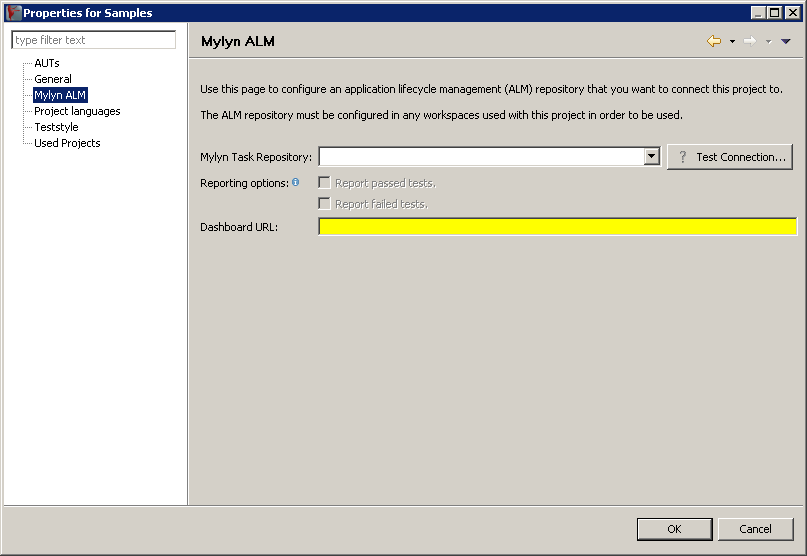
\includegraphics[width=12.5cm]{Tasks/ALM/PS/almproperties}
\caption{ALM Settings}
\label{TasksALMProjectProperties}
\end{center}
\end{figure}


\subsection{Adding task IDs to \gdjobs{}, \gdsuites{} and \gdcases{}}
\label{TasksALMAddTask}
You can add a task ID to \gdcases{}, \gdsuites{} and \gdjobs{} in your \gdproject{}. 

The task ID should be a valid ID in the repository that you have specified as the repository for this \gdproject{} \bxpref{TasksALMConfigureProject}. Adding the task ID to an item in your \gdproject{} means that this item is the relevant test for that task in your repository. When you activate the option, any test results for this item will be added as a comment to the task in the repository. The comment will include a link to the dashboard, in which the test result report can be viewed.

To add a task ID to a \gdcase{}, \gdsuite{} or \gdjob{}:
\begin{enumerate}
\item Open the item in the editor by double-clicking it.
\item In the \gdpropview{}, in the cell for \bxname{Task ID}, enter the task ID from the external repository. You can only enter task IDs at the place of specification -- you cannot overwrite them when you reuse the item.
\item Save the editor. 
\item When you have added a task ID to a node, you can open the task for this node from the browser by selecting:\\
\bxmenu{Open with}{Mylyn Task Editor}{}
\end{enumerate}

\bxtipp{You should ensure that you add task IDs to the right node-level to provide you with the relevant amount of information for the tasks in your repository. This will usually be at the level of Use Cases within a \gdsuite{}. }




\clearpage
\printindex
